\apendice{Especificación de diseño}

\section{Introducción}

Este anexo especifica la estructura de los datos, los procedimientos y la arquitectura del sistema. Además se incluyen los prototipados horizontales realizados tanto de baja como de alta fidelidad.

\section{Diseño de datos}

El diseño de datos es mostrado en esta sección detallando cada una de las tablas creadas y usadas por la plataforma web para almacenar y recuperar la información que el sistema mantiene.

\subsection{Base de Datos}

Este apartado especifican todas las tablas creadas para almacenar los datos del sistema en la Base de Datos así como el esquema final de las mismas que puede observarse en la Figura \ref{db-schema}.

\begin{figure}[!htbp]
  \centering
    \includegraphics[width=0.8\textwidth]{../img/db/db-schema.jpg}
  \caption{Esquema final de las tablas de la Base de Datos.}
  \label{db-schema}
\end{figure}

\subsubsection{tfm\_area}
La tabla \quotes{tfm\_area} permite almacenar las áreas a las que serán asignadas las distintas rutas almacenadas. Las columnas de esta tabla son las siguientes:

\begin{itemize}
	\item \textbf{id:} identificador de la tabla, es su clave primaria.
	\item \textbf{nombre:} contiene el nombre del área.
	\item \textbf{descripcion:} es la descripción que el usuario asigna al área.
	\item \textbf{min\_lat:} latitud mínima del área, por así decirlo, es su límite sur en un mapa.
	\item \textbf{min\_long:} longitud mínima, su límite oeste sobre un mapa.
	\item \textbf{max\_lat:} corresponde con la latitud máxima o su límite norte en el mapa.
	\item \textbf{max\_long:} la longitud máxima es el límite este sobre un mapa.
	\item \textbf{activa:} este valor booleano indica si el área está activa o no. Es decir, estando activa permite ser elegible como área asignable a rutas. Por defecto, su valor siempre será verdadero. 
	\item \textbf{fecha\_creacion:} marca temporal de creación del área.
	\item \textbf{fecha\_modificacion:} marca temporal de modificación de los valores de la misma.
\end{itemize}

\subsubsection{tfm\_nodos}
Tabla \quotes{tfm\_nodos}, almacena los nodos correspondientes a los Puntos De Interés. Sus columnas son las siguientes:

\begin{itemize}
	\item \textbf{id:} identificador primario de la tabla.
	\item \textbf{latitud:} latitud correspondiente a la ubicación del nodo.
	\item \textbf{longitud:} longitud que completa la coordenada geográfica correspondiente al nodo en cuestión.
	\item \textbf{nombre:} nombre que recibe el nodo.
	\item \textbf{the\_geom:} valor de geometría calculado y asignado por PostGIS.
	\item \textbf{id\_region:} referencia ajena a la tabla \quotes{tfm\_region\_pois}.
	\item \textbf{\textit{amenity:}} tipo de nodo (generalización).
\end{itemize}

\subsubsection{tfm\_caminos}
La tabla \quotes{tfm\_caminos} permite almacenar los valores de un camino presente en los ficheros xml correspondientes a los PDIs. Estas son sus columnas:

\begin{itemize}
	\item \textbf{id:} identificador del camino.
	\item \textbf{nodo:} identificador del nodo incluido en el camino.
	\item \textbf{tags:} etiquetas que contiene el camino. En este caso se almacenan los valores de las \textit{amenities}.
	\item \textbf{id\_region:} identificador de clave ajena que referencia a la tabla \quotes{tfm\_region\_pois}.
\end{itemize}

\subsubsection{tfm\_experimento}
\quotes{tfm\_experimento} almacena los valores que se han asociado a un experimento o prueba. Es decir, contiene todas las variables que el usuario ha elegido para lanzar una ejecución del algoritmo. Las columnas que contiene esta tabla son las siguientes:

\begin{itemize}
	\item \textbf{id\_experimento:} identificador primario de la tabla.
	\item \textbf{tipo\_asignacion\_area:} es la forma en la que el área ha sido asignada. Manual, seleccionando un área existente o creación de una nueva área.
	\item \textbf{id\_area\_asignada:} es el identificador del área asignada a las rutas.
	\item \textbf{buscar\_paradas:} este valor booleano indica si el usuario ha seleccionado la búsqueda de paradas durante el proceso de selección de opciones.
	\item \textbf{distancia\_parada:} es la distancia máxima a la que dos posiciones secuenciales se considerarán paradas.
	\item \textbf{variacion\_mediana:} multiplicador que permite realizar una variación sobre la mediana obtenida por el algoritmo.
	\item \textbf{buscar\_pois:} indica si el usuario ha deseado buscar PDIs en las rutas analizadas.
	\item \textbf{radio\_maximo:} es el valor que indica el radio máximo al que buscar PDIs sobre una parada.
	\item \textbf{mult\_radio:} el multiplicador del radio permite ampliar el rango espacial de la búsqueda de Puntos De Interés.
	\item \textbf{almacenado\_db:} es un valor booleano que indica si se ha almacenado la prueba en la Base de Datos.
	\item \textbf{fecha\_experimento:} la fecha en la que la prueba o ejecución del algoritmo ha tenido lugar.
	\item \textbf{nuevo:} variable booleana que toma valor verdadero para las últimas pruebas ejecutadas. Si el algoritmo se cancela por cualquier motivo, todas las pruebas marcadas como verdaderas serán eliminadas por seguridad.
	\item \textbf{es\_temporal:} indica si el usuario no ha deseado almacenar los datos en la Base de Datos. Esta variable será tomada para eliminar los datos de las tablas al cerrar el navegador.
	\item \textbf{distancia\_ruta:} este último valor indica la distancia máxima a la que una ruta se partirá en dos. El algoritmo tomará este valor junto a la mediana temporal calculada.
\end{itemize}

\subsubsection{tfm\_experimento\_fichero}
La tabla \quotes{tfm\_experimento\_fichero} almacena dos identificadores hacia sendas tablas, estas tablas son: \quotes{tfm\_experimento} y \quotes{tfm\_fichero}. De esta forma se puede  conocer qué ficheros han sido analizados en la prueba ejecutada.

\subsubsection{tfm\_experimento\_ruta}
La tabla \quotes{tfm\_experimento\_ruta} almacena otros dos identificadores ligados a las tablas \quotes{tfm\_experimento} y \quotes{tfm\_ruta}. Por tanto, mediante estos identificadores, se podrá conocer cuáles han sido las rutas creadas durante la ejecución de la prueba.

\subsubsection{tfm\_fichero}
\quotes{tfm\_fichero} almacena los datos referentes a los ficheros de rutas subidos al servidor. Esta tabla cuenta con las siguientes columnas:

\begin{itemize}
	\item \textbf{id\_fichero:} identificador primario de la tabla.
	\item \textbf{nombre:} nombre del fichero subido.
	\item \textbf{fecha\_subida:} fecha en la que el fichero ha sido subido.
	\item \textbf{procesado:} variable booleana que indica si el fichero ha sido seleccionado en alguna ejecución del algoritmo.
	\item \textbf{fecha\_procesado:} en caso de que la variable anterior sea positiva, la fecha tomará el valor de la ejecución del algoritmo.
\end{itemize}

\subsubsection{tfm\_fichero\_poi}
La tabla \quotes{tfm\_fichero\_poi} almacena los nombres y fechas de procesado de los ficheros de Puntos De Interés. Sus columnas son:

\begin{itemize}
	\item \textbf{id\_fichero:} es un identificador primario de la tabla.
	\item \textbf{nombre:} contiene el nombre del fichero analizado.
	\item \textbf{fecha\_procesado:} indica la fecha en la que el fichero ha sido procesado.
\end{itemize}

\subsubsection{tfm\_nombre\_nodo}
Esta tabla, \quotes{tfm\_nombre\_nodo}, indica los nombres (amenities) de los nodos que son leídos durante el proceso de \textit{parseo} de un fichero de PDIs. Las columnas son:

\begin{itemize}
	\item \textbf{id\_nombre:} es el identificador primario de la tabla.
	\item \textbf{nombre:} es el nombre que recibe la amenity del nodo.
\end{itemize}

\subsubsection{tfm\_posicion}
La tabla \quotes{tfm\_posicion} permite almacenar los valores de las posiciones que contiene cada ruta. Las columnas de la tabla son las siguientes:

\begin{itemize}
	\item \textbf{id\_posicion:} identificador primario de la posición.
	\item \textbf{id\_ruta:} identificador de clave ajena a la ruta.
	\item \textbf{latitud:} latitud de la coordenada geográfica.
	\item \textbf{longitud:} longitud de la coordenada geográfica.
	\item \textbf{date\_time:} marca temporal de la posición.
	\item \textbf{altitud:} valor que indica la altitud de la posición.
	\item \textbf{the\_geom:} valor de tipo \quotes{geometry} que permite ubicar la posición a PostGIS.
	\item \textbf{es\_parada:} es una variable booleana que indica si la posición forma parte de una parada.
\end{itemize}

\subsubsection{tfm\_posicion\_poi}
La tabla \quotes{tfm\_posicion\_poi} permite mantener una relación entre nodos y posiciones, siempre que estas sean una parada en la ruta. Las columnas que definen esta tabla son:

\begin{itemize}
	\item \textbf{id\_posicion\_poì:} identificador primario de la tabla.
	\item \textbf{id\_nodo:} identificador del nodo.
	\item \textbf{distancia:} distancia calculada a la posición.
	\item \textbf{id\_posicion\_poi:} identificador primario.
\end{itemize}

\subsubsection{tfm\_proceso\_poi}
\quotes{tfm\_proceso\_poi} mantiene un índice en una sola fila que indica el paso en el que el procesado de PDIs se encuentra. Contiene estas columnas:

\begin{itemize}
	\item \textbf{id\_proceso\_poi:} identificador primario.
	\item \textbf{estado:} valor entero.
\end{itemize}

\subsubsection{tfm\_proceso\_ruta}
De la misma forma que la tabla anterior contiene información sobre el estado de proceso de PDIs, esta tabla realiza lo propio con el algoritmo de análisis de rutas:

\begin{itemize}
	\item \textbf{id\_proceso\_ruta:} identificador primario de la tabla.
	\item \textbf{estado:} estado en el que se encuentra el algoritmo.
\end{itemize}

\subsubsection{tfm\_region\_pois}
La tabla \quotes{tfm\_region\_pois} almacena la región que forma cada fichero procesado. Sus columnas son:

\begin{itemize}
	\item \textbf{id\_region:} es el identificador primario de esta tabla.
	\item \textbf{nombre:} es una cadena que almacena el nombre de la región a la que pertenecen los PDIs de cada uno de los ficheros procesados.
\end{itemize}

\subsubsection{tfm\_ruta}
La tabla \quotes{tfm\_ruta} almacena todos los datos relativos a las rutas. Sus campos son:

\begin{itemize}
	\item \textbf{id\_ruta:} identificador primario de la ruta.
	\item \textbf{id\_usuario:} identificador de clave ajena hacia la tabla de usuarios.
	\item \textbf{id\_area:} identificador de clave ajena hacia la tabla de áreas.
	\item \textbf{fecha\_creacion:} es la fecha de creación de la ruta en la Base de Datos.
	\item \textbf{nuevo:} indica si la ruta es nueva, podrá ser consultado para eliminar todas las rutas en caso de que la ejecución sea detenida.
	\item \textbf{es\_temporal:} indica si el usuario no ha querido guardar la ruta de forma permanente  y será eliminada
	\item \textbf{fecha\_comienzo:} es la fecha de comienzo de la ruta analizada. Esta fecha permite conocer el dato  de comienzo sin tener que obtener las posiciones de la ruta.
	\item \textbf{fecha\_fin:} valor de fecha en la que la ruta finaliza.
\end{itemize}

\subsubsection{tfm\_ruta\_area}
La tabla \quotes{tfm\_ruta\_area} almacena, a modo de caché, el área que forma cada una de las rutas analizadas. De esta forma se pueden obtener rutas que pueden pertenecer a una o varias áreas. Las columnas son:

\begin{itemize}
	\item \textbf{id\_ruta:} identificador de de clave ajena a las rutas.
	\item \textbf{min\_lat:} latitud mínima del área que engloba a la ruta.
	\item \textbf{min\_long:} longitud mínima del área que engloba a la ruta.
	\item \textbf{max\_lat:} latitud máxima del área que engloba a la ruta.
	\item \textbf{max\_long:} longitud máxima del área que engloba a la ruta.
	\item \textbf{id\_ruta\_area:} identificador primario de la tabla.
\end{itemize}

\subsubsection{tfm\_usuario}
La tabla \quotes{tfm\_usuario} puede mantener un listado de usuarios en base a sus identificadores. En el caso de este trabajo, se mantendrá un único usuario puesto que no se cuenta con una gestión de usuarios. En futuras revisiones del trabajo, la gestión de usuarios podrá ser una alternativa interesante a desarrollar.

\begin{itemize}
	\item \textbf{id\_usuario:} es el identificador único de usuario.
\end{itemize}

\section{Diseño procedimental}

El diseño procedimental forma parte del proceso de diseño de software. Este diseño se realiza una vez establecida la estructura de la aplicación y de sus datos.
A continuación se mostrarán los diagramas de secuencias necesarios para comprender el comportamiento de la aplicación.

\section{Diseño arquitectónico}
Este apartado del Anexo de Diseño refleja el diseño arquitectónico de la aplicación implementada. A continuación se muestra al arquitectura y la estructura de paquetes.


\subsection{Diagramas de secuencias}
Este apartado muestra los diagramas de secuencias \cite{seq:info}.

\subsubsection{Subida de ficheros}
Diagrama de secuencias para la subida de un fichero de datos a la plataforma. Figura \ref{subida}.

\begin{figure}[!htbp]
  \centering
    \includegraphics[width=0.8\textwidth]{../img/diagramas/secuencias/4.jpg}
  \caption{Diagrama de secuencias de subida de ficheros a la plataforma.}
  \label{subida}
\end{figure}

\subsubsection{Borrado de datos}
Diagrama de secuencias para el borrado de datos. Figura \ref{borradodatos}.
\begin{figure}[!htbp]
  \centering
    \includegraphics[width=0.8\textwidth]{../img/diagramas/secuencias/2.jpg}
  \caption{Borrado de datos en el sistema.}
  \label{borradodatos}
\end{figure}

\subsubsection{Borrado de ficheros}
Diagrama de secuencias para el borrado de ficheros. Figura \ref{borradoficheros}.
\begin{figure}[!htbp]
  \centering
    \includegraphics[width=0.8\textwidth]{../img/diagramas/secuencias/1.jpg}
  \caption{Diagrama de secuencias de borrado de fichreos.}
  \label{borradoficheros}
\end{figure}

\subsubsection{Subir ficheros de PDIs}
Diagrama de secuencias para la subida de ficheros de PDIs. Figura \ref{subidapdis}.
\begin{figure}[!htbp]
  \centering
    \includegraphics[width=0.8\textwidth]{../img/diagramas/secuencias/3.jpg}
  \caption{Diagrama de secuencias de subida de ficheros de PDIs.}
  \label{subidapdis}
\end{figure}

\subsubsection{Borrar región}
Diagrama de secuencias para borrar regiones. Figura \ref{borradoregion}.
\begin{figure}[!htbp]
  \centering
    \includegraphics[width=0.8\textwidth]{../img/diagramas/secuencias/5.jpg}
  \caption{Borrado de región.}
  \label{borradoregion}
\end{figure}

\subsubsection{Crear área}
Diagrama de secuencias para crear áreas. Figrua \ref{creacionarea}.
\begin{figure}[!htbp]
  \centering
    \includegraphics[width=0.8\textwidth]{../img/diagramas/secuencias/6.jpg}
  \caption{Diagrama de secuencias de la creación de áreas.}
  \label{creacionarea}
\end{figure}

\subsubsection{Pruebas}
Diagrama de secuencias para recuperar las pruebas realizadas.
\begin{figure}[!htbp]
  \centering
    \includegraphics[width=0.8\textwidth]{../img/diagramas/secuencias/11.jpg}
  \caption{Recuperación de pruebas.}
  \label{recprueba}
\end{figure}

\subsubsection{Repetir prueba}
Diagrama de secuencias para repetir una prueba. Figura \ref{repprueba}, se continua en \quotes{Procesado de ficheros}.
\begin{figure}[!htbp]
  \centering
    \includegraphics[width=0.8\textwidth]{../img/diagramas/secuencias/13.jpg}
  \caption{Repetición de prueba.}
  \label{repprueba}
\end{figure}

\subsubsection{Borrar prueba}
Diagrama de secuencias para borrar una prueba realizada. Figura \ref{borradoprueba}.
\begin{figure}[!htbp]
  \centering
    \includegraphics[width=0.8\textwidth]{../img/diagramas/secuencias/12.jpg}
  \caption{Borrado de pruebas.}
  \label{borradoprueba}
\end{figure}

\subsubsection{Resultados}
Diagrama de secuencias para recuperar los resultados obtenidos del análisis de datos. Figura \ref{resultados}.
\begin{figure}[!htbp]
  \centering
    \includegraphics[width=0.8\textwidth]{../img/diagramas/secuencias/14.jpg}
  \caption{Diagrama de secuencias de obtención de resultados.}
  \label{resultados}
\end{figure}

\subsubsection{Lectura de ficheros}
Diagrama de secuencias para leer ficheros, generación de una ruta inicial y su posterior procesado. Figura \ref{lectura}, continua en \quotes{Procesado de Rutas}.
\begin{figure}[!htbp]
  \centering
    \includegraphics[width=0.8\textwidth]{../img/diagramas/secuencias/7.jpg}
  \caption{Lectura de ficheros.}
  \label{lectura}
\end{figure}

\subsubsection{Procesado de Rutas}
Diagrama de secuencias para procesar las rutas leídas en el procesado de ficheros. Figura \ref{procesado}, se continua con el \quotes{Procesado de paradas}.
\begin{figure}[!htbp]
  \centering
    \includegraphics[width=0.8\textwidth]{../img/diagramas/secuencias/8.jpg}
  \caption{Procesado de rutas.}
  \label{procesado}
\end{figure}

\subsubsection{Procesado de Paradas}
Diagrama de secuencias para procesar las paradas de las rutas detectadas en el paso anterior. La Figura \ref{paradas} lo muestra, continua en \quotes{Procesado de PDIs}.
\begin{figure}[!htbp]
  \centering
    \includegraphics[width=0.8\textwidth]{../img/diagramas/secuencias/9.jpg}
  \caption{Procesado de paradas en las rutas.}
  \label{paradas}
\end{figure}

\subsubsection{Procesado de PDIs}
Diagrama de secuencias para obtener los PDIs cercanos a las paradas que han sido detectadas. También se muestra el almacenado en la Base de Datos. Figura \ref{pdis}.
\begin{figure}[!htbp]
  \centering
    \includegraphics[width=0.8\textwidth]{../img/diagramas/secuencias/10.jpg}
  \caption{Diagrama de secuencias de procesado de PDIs.}
  \label{pdis}
\end{figure}


\subsection{Arquitectura MVC}

El proyecto de esta plataforma web sigue el patrón arquitectónico Modelo-Vista-Controlador \cite{mvc:wiki}. Este patrón, generalmente, es usado para el diseño de aplicaciones que requieren de una interfaz de usuario permitiendo separar la lógica de negocio de la interfaz o vista y, por último, de los datos. La gran mayoría de \textit{frameworks} de desarrollo web usan esta arquitectura.

El diagrama de esta arquitectura es el mostrado en la Figura \ref{mvc}. Como se aprecia en la imagen, la arquitectura está separada en tres componentes:

\begin{itemize}
	\item \textbf{Controlador:} el controlador responde a los eventos que le requiera el usuario. De esta forma es el encargado de llamar al modelo cuando se solicita algún tipo de tratamiento de información. También puede interactuar con la vista para cambiar la forma en que la interfaz se muestra al usuario. Se puede decir que el controlador es un intermediario entre la vista y el modelo.
	\item \textbf{Vista:} la vista presenta la información al usuario correctamente formateada.
	\item \textbf{Modelo:} el modelo es una representación de los datos con los que trabaja el sistema. En Java se puede asimilar con las clases que representan cada uno de los objetos. También contiene la lógica de negocio que permite el acceso y manipulación de los datos.
\end{itemize}

Este comportamiento se puede definir de la siguiente forma:

\begin{enumerate}
	\item \textbf{Petición del usuario al controlador:} la interacción comienza cuando el usuario realiza una petición al controlador.
	\item \textbf{Solicitud de datos:} el controlador realizará una petición al modelo para solicitar los datos requeridos por el usuario.
	\item \textbf{Devolución de datos:} el modelo devuelve los datos al controlador.
	\item \textbf{Llamada a una vista:} en este momento, el controlador buscará la vista adecuada para representar la información.
	\item \textbf{Se devuelve la vista al controlador:} una vez la vista es seleccionada, es devuelta al controlador que realizará el último paso.
	\item \textbf{Devolución de la vista al usuario:} por último, la vista es devuelta con la información solicitada al usuario. En este caso, la vista se representará en el navegador web.
\end{enumerate}

\begin{figure}[!htbp]
  \centering
    \includegraphics[width=0.8\textwidth]{../img/mvc/mvc.png}
  \caption{Esquema general de la arquitectura MVC.}
  \label{mvc}
\end{figure}

\subsection{Arquitectura web}
La arquitectura web elegida ha sido \textit{Java Server Pages} conocida como JSP. Esta arquitectura permite crear páginas web dinámicas por medio de las clases Java que se almacenan en el servidor.

Como se comenta en otras secciones de la guía, esta arquitectura fue elegida una vez comenzado el proyecto debido a que ha permitido reutilizar todo el código implementado con anterioridad puesto que se usan clases Java estándar. La Figura  \ref{jsp} permite ver cómo es una arquitectura JSP estándar como la usada en el presente proyecto.

\begin{figure}[!htbp]
  \centering
    \includegraphics[width=0.5\textwidth]{../img/jsp/jsp.png}
  \caption{Arquitectura estándar de JSP.}
  \label{jsp}
\end{figure}

\subsection{Estructura de paquetes del sistema}
En este apartado se muestra la estructura de paquetes con la que cuenta el proyecto. Debido al uso de la arquitectura MVC se separan en tres grandes bloques.

\subsubsection{Modelo}
Los clases incluidas en el sub paquete \quotes{Model} se dividen a su vez en otros dos sub paquetes:

\begin{itemize}
	\item \textit{Dao}: paquete con las clases de acceso a datos (Data Access Object) que permiten las operaciones CRUD sobre la Base de Datos. Figura \ref{dao}.
	\item \textit{Data}: modelo de objetos de la aplicación web. Figura \ref{data}.
\end{itemize}

\begin{figure}[!htbp]
  \centering
    \includegraphics[width=0.8\textwidth]{../img/diagramas/model/dao/uno.jpg}
  \caption{Sub paquete \textit{dao} dentro del paquete \textit{model}.}
  \label{dao}
\end{figure}

\begin{figure}[!htbp]
  \centering
    \includegraphics[width=0.8\textwidth]{../img/diagramas/model/data/uno.jpg}
  \caption{Sub paquete \textit{data} dentro del paquete \textit{model}.}
  \label{data}
\end{figure}


\subsubsection{Controlador}
Los clases incluidas en el sub paquete \quotes{Controller} se dividen en tres sub paquetes adicionales.

\begin{itemize}
	\item \textit{Algorithm}: paquete que contiene las clases relacionadas con el algoritmo de análisis de rutas. Figura \ref{algorithm}.
	\item \textit{Connetion}: contiene las clases que permiten realizar una conexión contra la Base de Datos así como su configuración. Figura \ref{connection}.
	\item \textit{Servlet}: estas clases manejan el comportamiento de la plataforma web. Figura \ref{servlet}.
		\begin{itemize}
			\item \textit{utils}: utilidades para el manejo y/o control de hilos, obtención de identificadores de la Base de Datos, etc. Figura \ref{util}.
		\end{itemize}
\end{itemize}

\begin{figure}[!htbp]
  \centering
    \includegraphics[width=0.8\textwidth]{../img/diagramas/controller/algoritmo/uno.jpg}
  \caption{Sub paquete \textit{algorithm} del paquete \textit{controller}.}
  \label{algorithm}
\end{figure}

\begin{figure}[!htbp]
  \centering
    \includegraphics[width=0.8\textwidth]{../img/diagramas/controller/conexion/uno.jpg}
  \caption{Sub paquete \textit{connection} dentro del paquete \textit{controller}.}
  \label{connection}
\end{figure}

\begin{figure}[!htbp]
  \centering
    \includegraphics[width=0.8\textwidth]{../img/diagramas/controller/servlet/cuatro.jpg}
  \caption{Sub paquete \textit{servlet} en el paquete \textit{controller}.}
  \label{servlet}
\end{figure}


\begin{figure}[!htbp]
  \centering
    \includegraphics[width=0.8\textwidth]{../img/diagramas/controller/servlet/tres.jpg}
  \caption{Sub paquete \textit{utils} en el interior del paquete \textit{utils}.}
  \label{util}
\end{figure}



\subsubsection{Vista}
Las vistas están formadas por páginas de tipo jsp. Por tanto, no se puede mostrar un esquema de paquetes como el mostrado anteriormente. Destacar que la página principal se encuentra en la carpeta raíz y el resto de páginas bajo la carpeta \textit{pages}.


\section{Prototipado de la aplicación web}

La aplicación web sigue los conceptos descritos por Hassan-Montero \cite{montero:info} en relación al diseño web centrado en el usuario. Este apartado incluye los prototipados realizados.

\subsection{Prototipado horizontal de baja fidelidad}
Este prototipado muestra un primer diseño de la aplicación donde pueden verse algunas de las páginas planteadas en una primera aproximación. La lista de figuras mostradas corresponden con:

\begin{itemize}
	\item Figura \ref{principal}: muestra el posible aspecto de la portada de la plataforma web.
	\item Figura \ref{subida}: pretende mostrar la forma de la página de subida de ficheros.
	\item Figura \ref{ficheros}: visualiza el cómo se verá la página de selección de ficheros y opciones de ejecución del algoritmo.
	\item Figura \ref{encurso}: esta página será mostrada cuando un algoritmo se encuentre en ejecución.
	\item Figura \ref{mapa}: para visualizar de mejor forma una ruta, se podrán obtener sus valores característicos y ser mostrada sobre un mapa.
	\item Figura \ref{pruebas}: la página de pruebas mostrará las ejecuciones del algoritmo así como los valores con los que fueron realizadas.
	\item Figura \ref{gestion}: es una página de gestión de la plataforma web.
	\item Figura \ref{areas}: la página de gestión de áreas permite mantener las áreas disponibles en el sistema.
	\item Figura \ref{pdis}: esta página realiza la misma tarea que la descrita en el punto anterior pero se encuentra relacionada con los PDIs.
\end{itemize}

\begin{figure}[!htbp]
  \centering
    \includegraphics[width=0.8\textwidth]{../img/prototipado/baja/principal.png}
  \caption{Página principal.}
  \label{principal}
\end{figure}

\begin{figure}[!htbp]
  \centering
    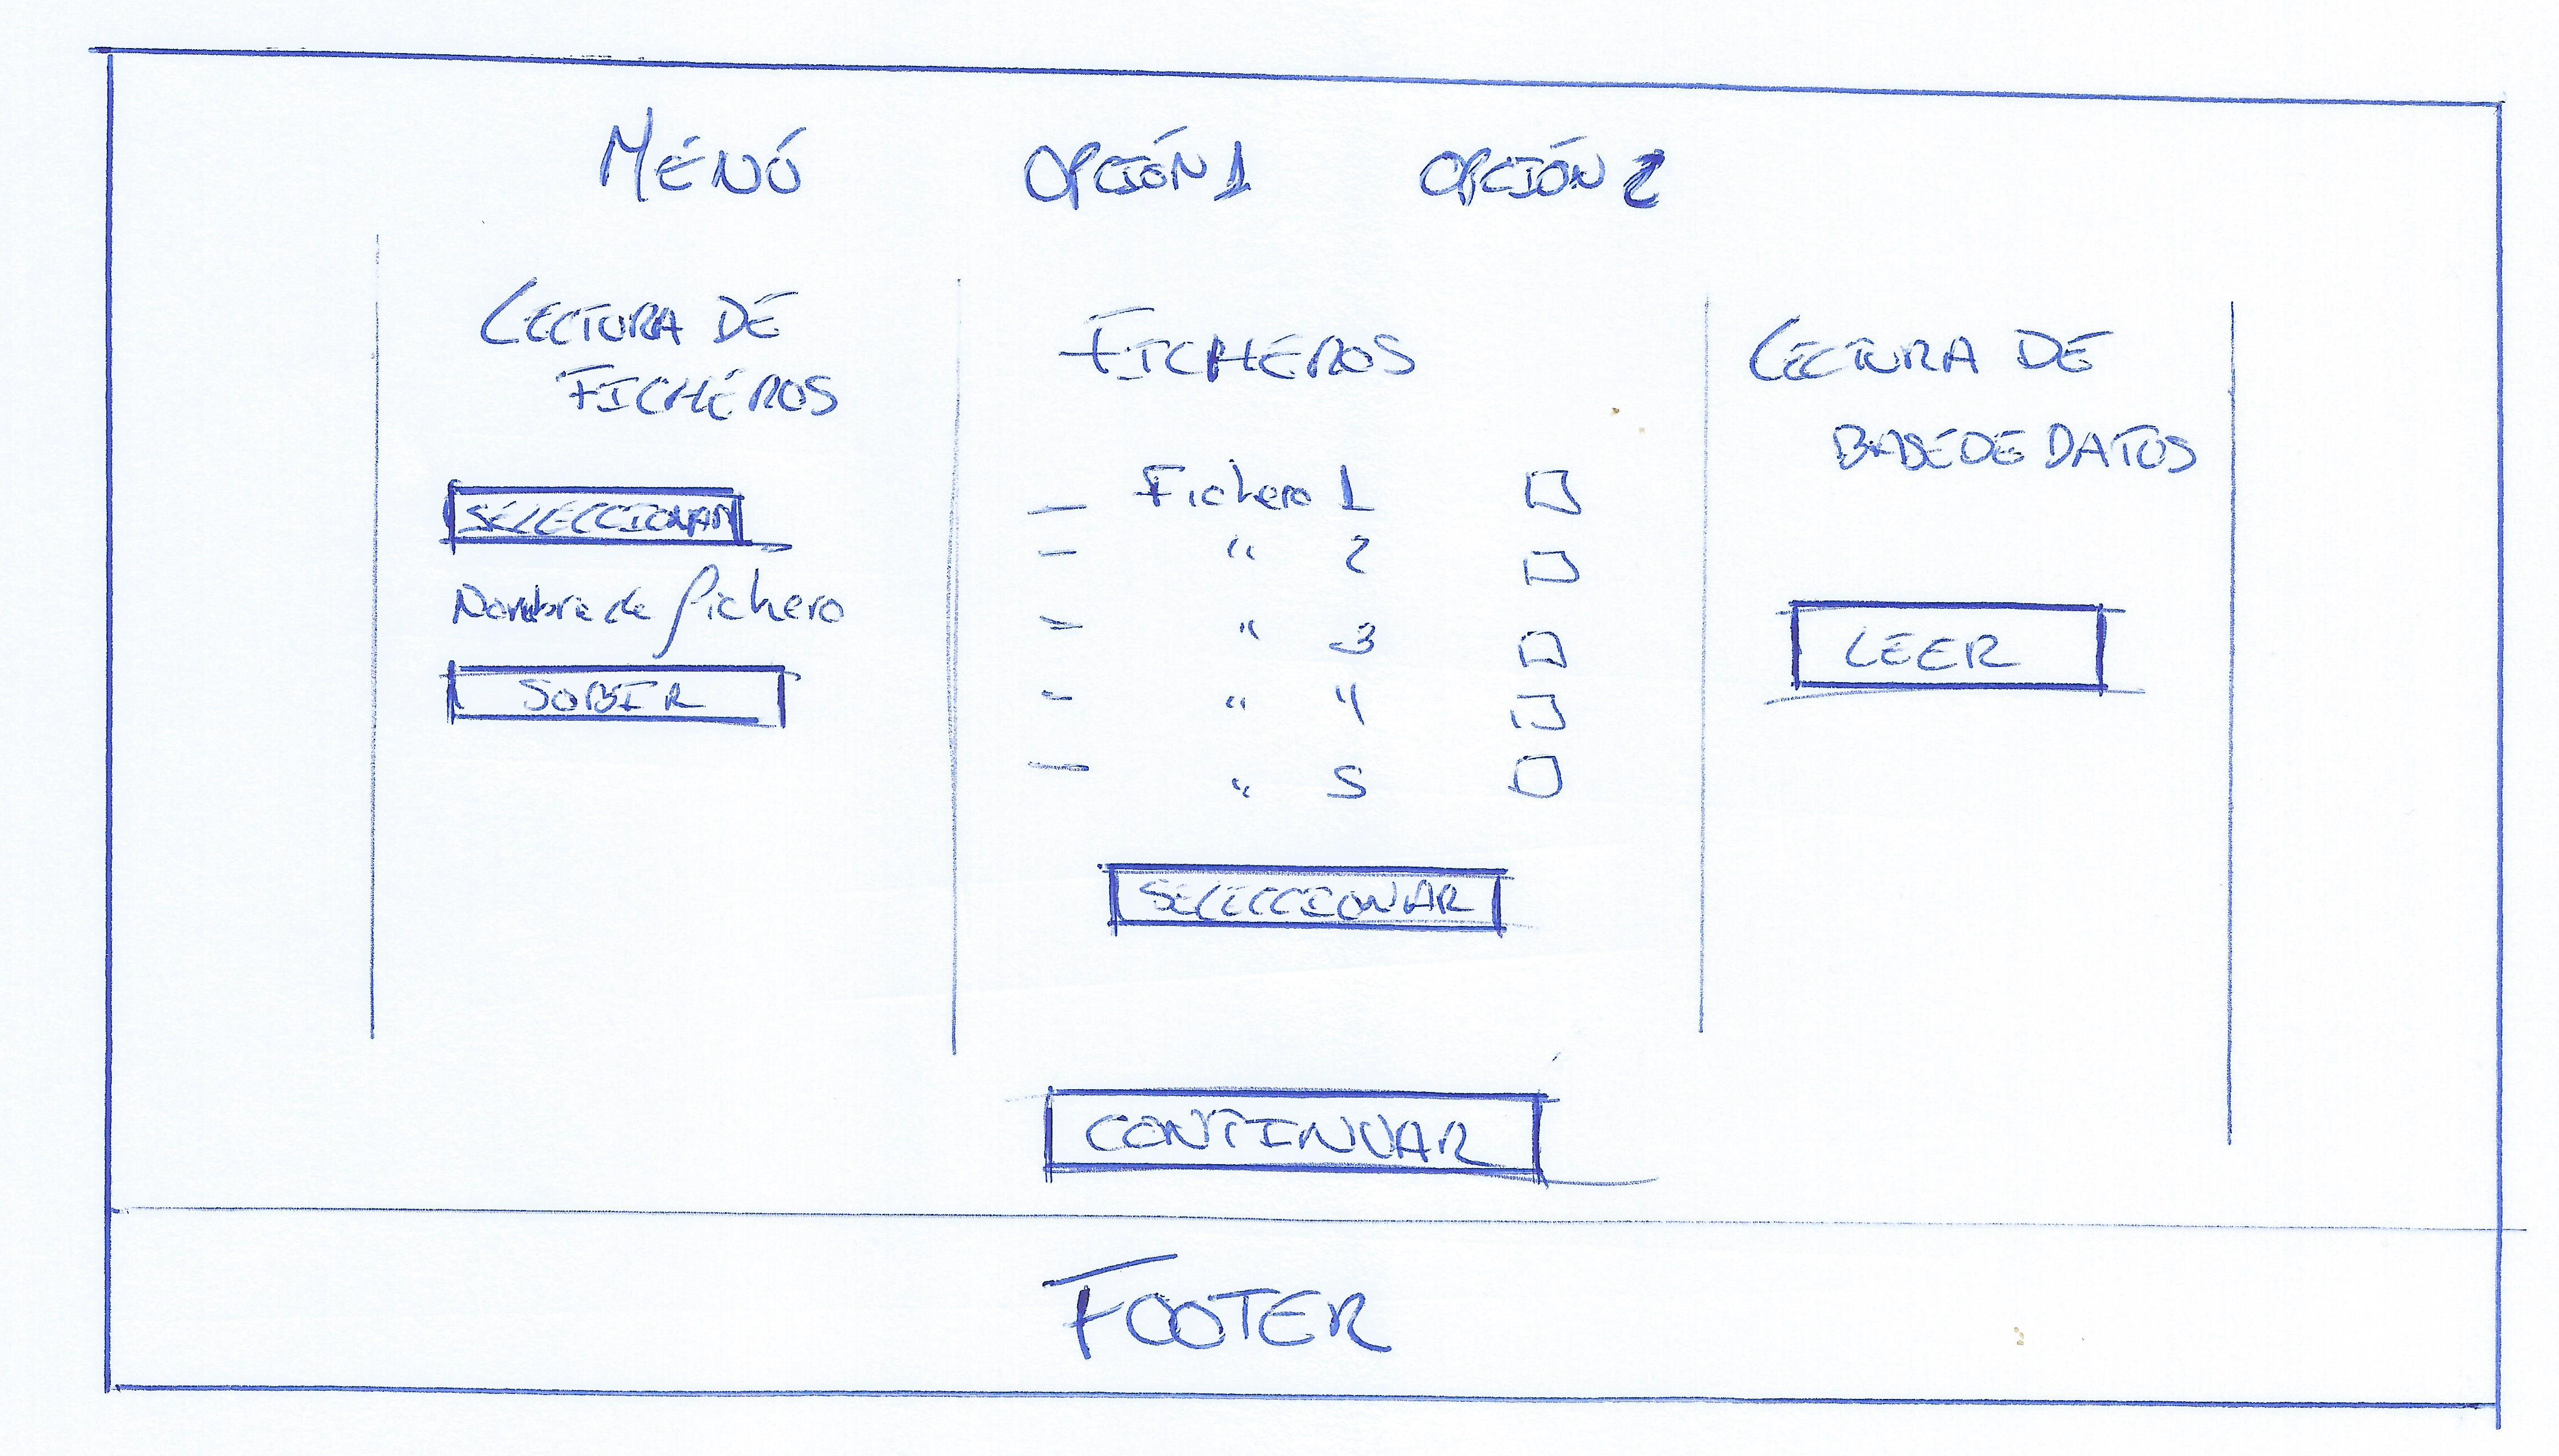
\includegraphics[width=0.8\textwidth]{../img/prototipado/baja/subida.png}
  \caption{Subida de ficheros.}
  \label{subida}
\end{figure}

\begin{figure}[!htbp]
  \centering
    \includegraphics[width=0.8\textwidth]{../img/prototipado/baja/ficheros.png}
  \caption{Selección de ficheros.}
  \label{ficheros}
\end{figure}

\begin{figure}[!htbp]
  \centering
    \includegraphics[width=0.8\textwidth]{../img/prototipado/baja/encurso.png}
  \caption{Algoritmo en curso.}
  \label{encurso}
\end{figure}

\begin{figure}[!htbp]
  \centering
    \includegraphics[width=0.8\textwidth]{../img/prototipado/baja/mapa.png}
  \caption{Mapa de ruta.}
  \label{mapa}
\end{figure}

\begin{figure}[!htbp]
  \centering
    \includegraphics[width=0.8\textwidth]{../img/prototipado/baja/pruebas.png}
  \caption{Pruebas realizadas.}
  \label{pruebas}
\end{figure}

\begin{figure}[!htbp]
  \centering
    \includegraphics[width=0.8\textwidth]{../img/prototipado/baja/gestion.png}
  \caption{Gestión principal.}
  \label{gestion}
\end{figure}

\begin{figure}[!htbp]
  \centering
    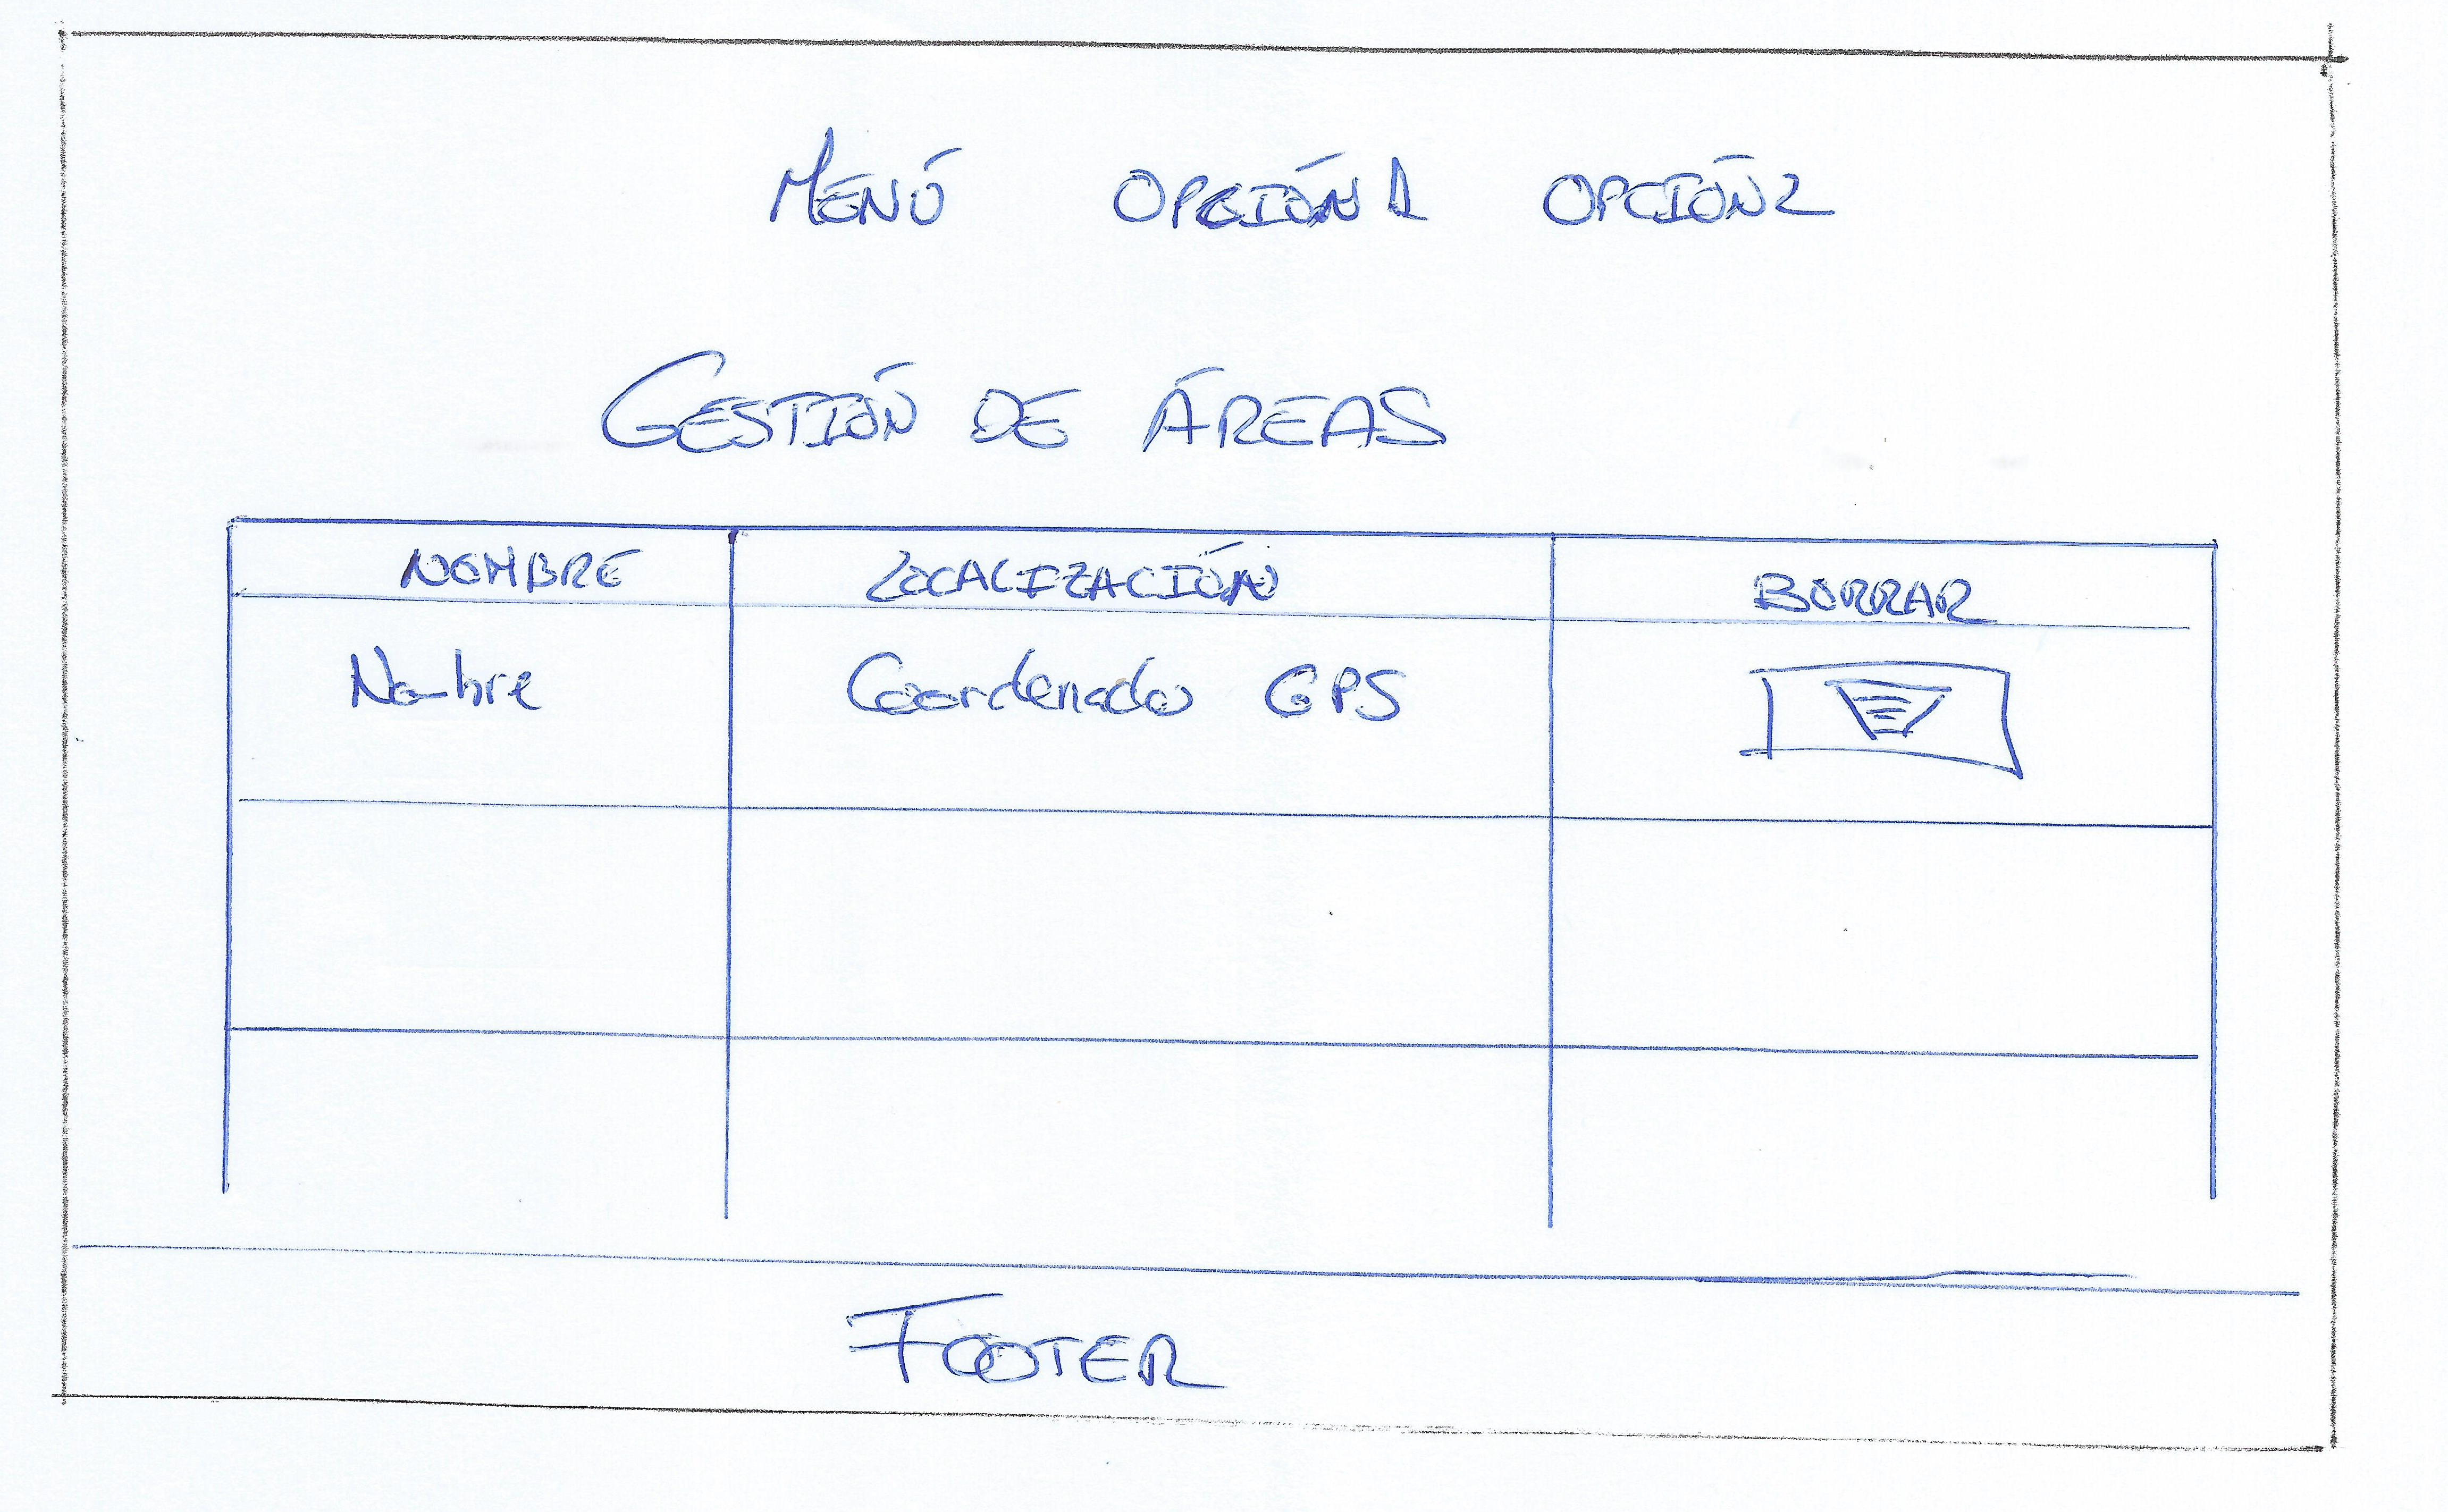
\includegraphics[width=0.8\textwidth]{../img/prototipado/baja/areas.png}
  \caption{Gestión de áreas.}
  \label{areas}
\end{figure}

\begin{figure}[!htbp]
  \centering
    \includegraphics[width=0.8\textwidth]{../img/prototipado/baja/pdis.png}
  \caption{Gestión de PDIs.}
  \label{pdis}
\end{figure}

\subsection{Prototipado horizontal de alta fidelidad} 
El prototipado de alta fidelidad muestra el aspecto final que tomará la plataforma web. La siguiente lista de figuras detalla cada una de las páginas mostradas:

\begin{itemize}
	\item Figura \ref{principal}: es la portada de la aplicación.
	\item Figura \ref{sinficheros}: este aspecto será mostrado si el sistema no cuenta con ficheros.
	\item Figura \ref{gestionficheros}: esa una página que permite gestionar los ficheros en la plataforma.
	\item Figura \ref{algoritmo}: son las opciones de procesado del algoritmo disponibles para el usuario.
	\item Figura \ref{encurso}: prueba en curso.
	\item Figura \ref{ejecucionfin}: prueba finalizada.
	\item Figura \ref{datosdisponibles}: al finalizar una ejecución pueden verse los resultados en esta página.
	\item Figura \ref{ayuda}: todas las páginas cuentan con ayuda para el usuario.
	\item Figura \ref{mapas}: si se desea ver una ruta en detalle, se puede ver en un mapa.
	\item Figura \ref{pruebas}: la página de pruebas muestra las ejecuciones que se han realizado del algoritmo.
	\item Figura \ref{borradopruebas}: se permite el borrado de pruebas tal como se aprecia en la imagen.
	\item Figura \ref{gestion}: la página principal de gestión permite acceder a páginas secundarias.
	\item Figura \ref{areasdispo}: son las áreas disponibles, también permite crear, modificar o eliminar un área.
	\item Figura \ref{nuevaarea}: este formulario permite la creación de un área.
	\item Figura \ref{pdis}: muestra los PDIs del sistemas así como un formulario de subida de ficheros.
	\item Figura \ref{borrado}:	esta es la página de borrado de datos de la aplicación web.	
\end{itemize}

\begin{figure}[!htbp]
  \centering
    \includegraphics[width=0.8\textwidth]{../img/prototipado/alta/principal.png}
  \caption{Página principal de la aplicación web.}
  \label{principal}
\end{figure}

\begin{figure}[!htbp]
  \centering
    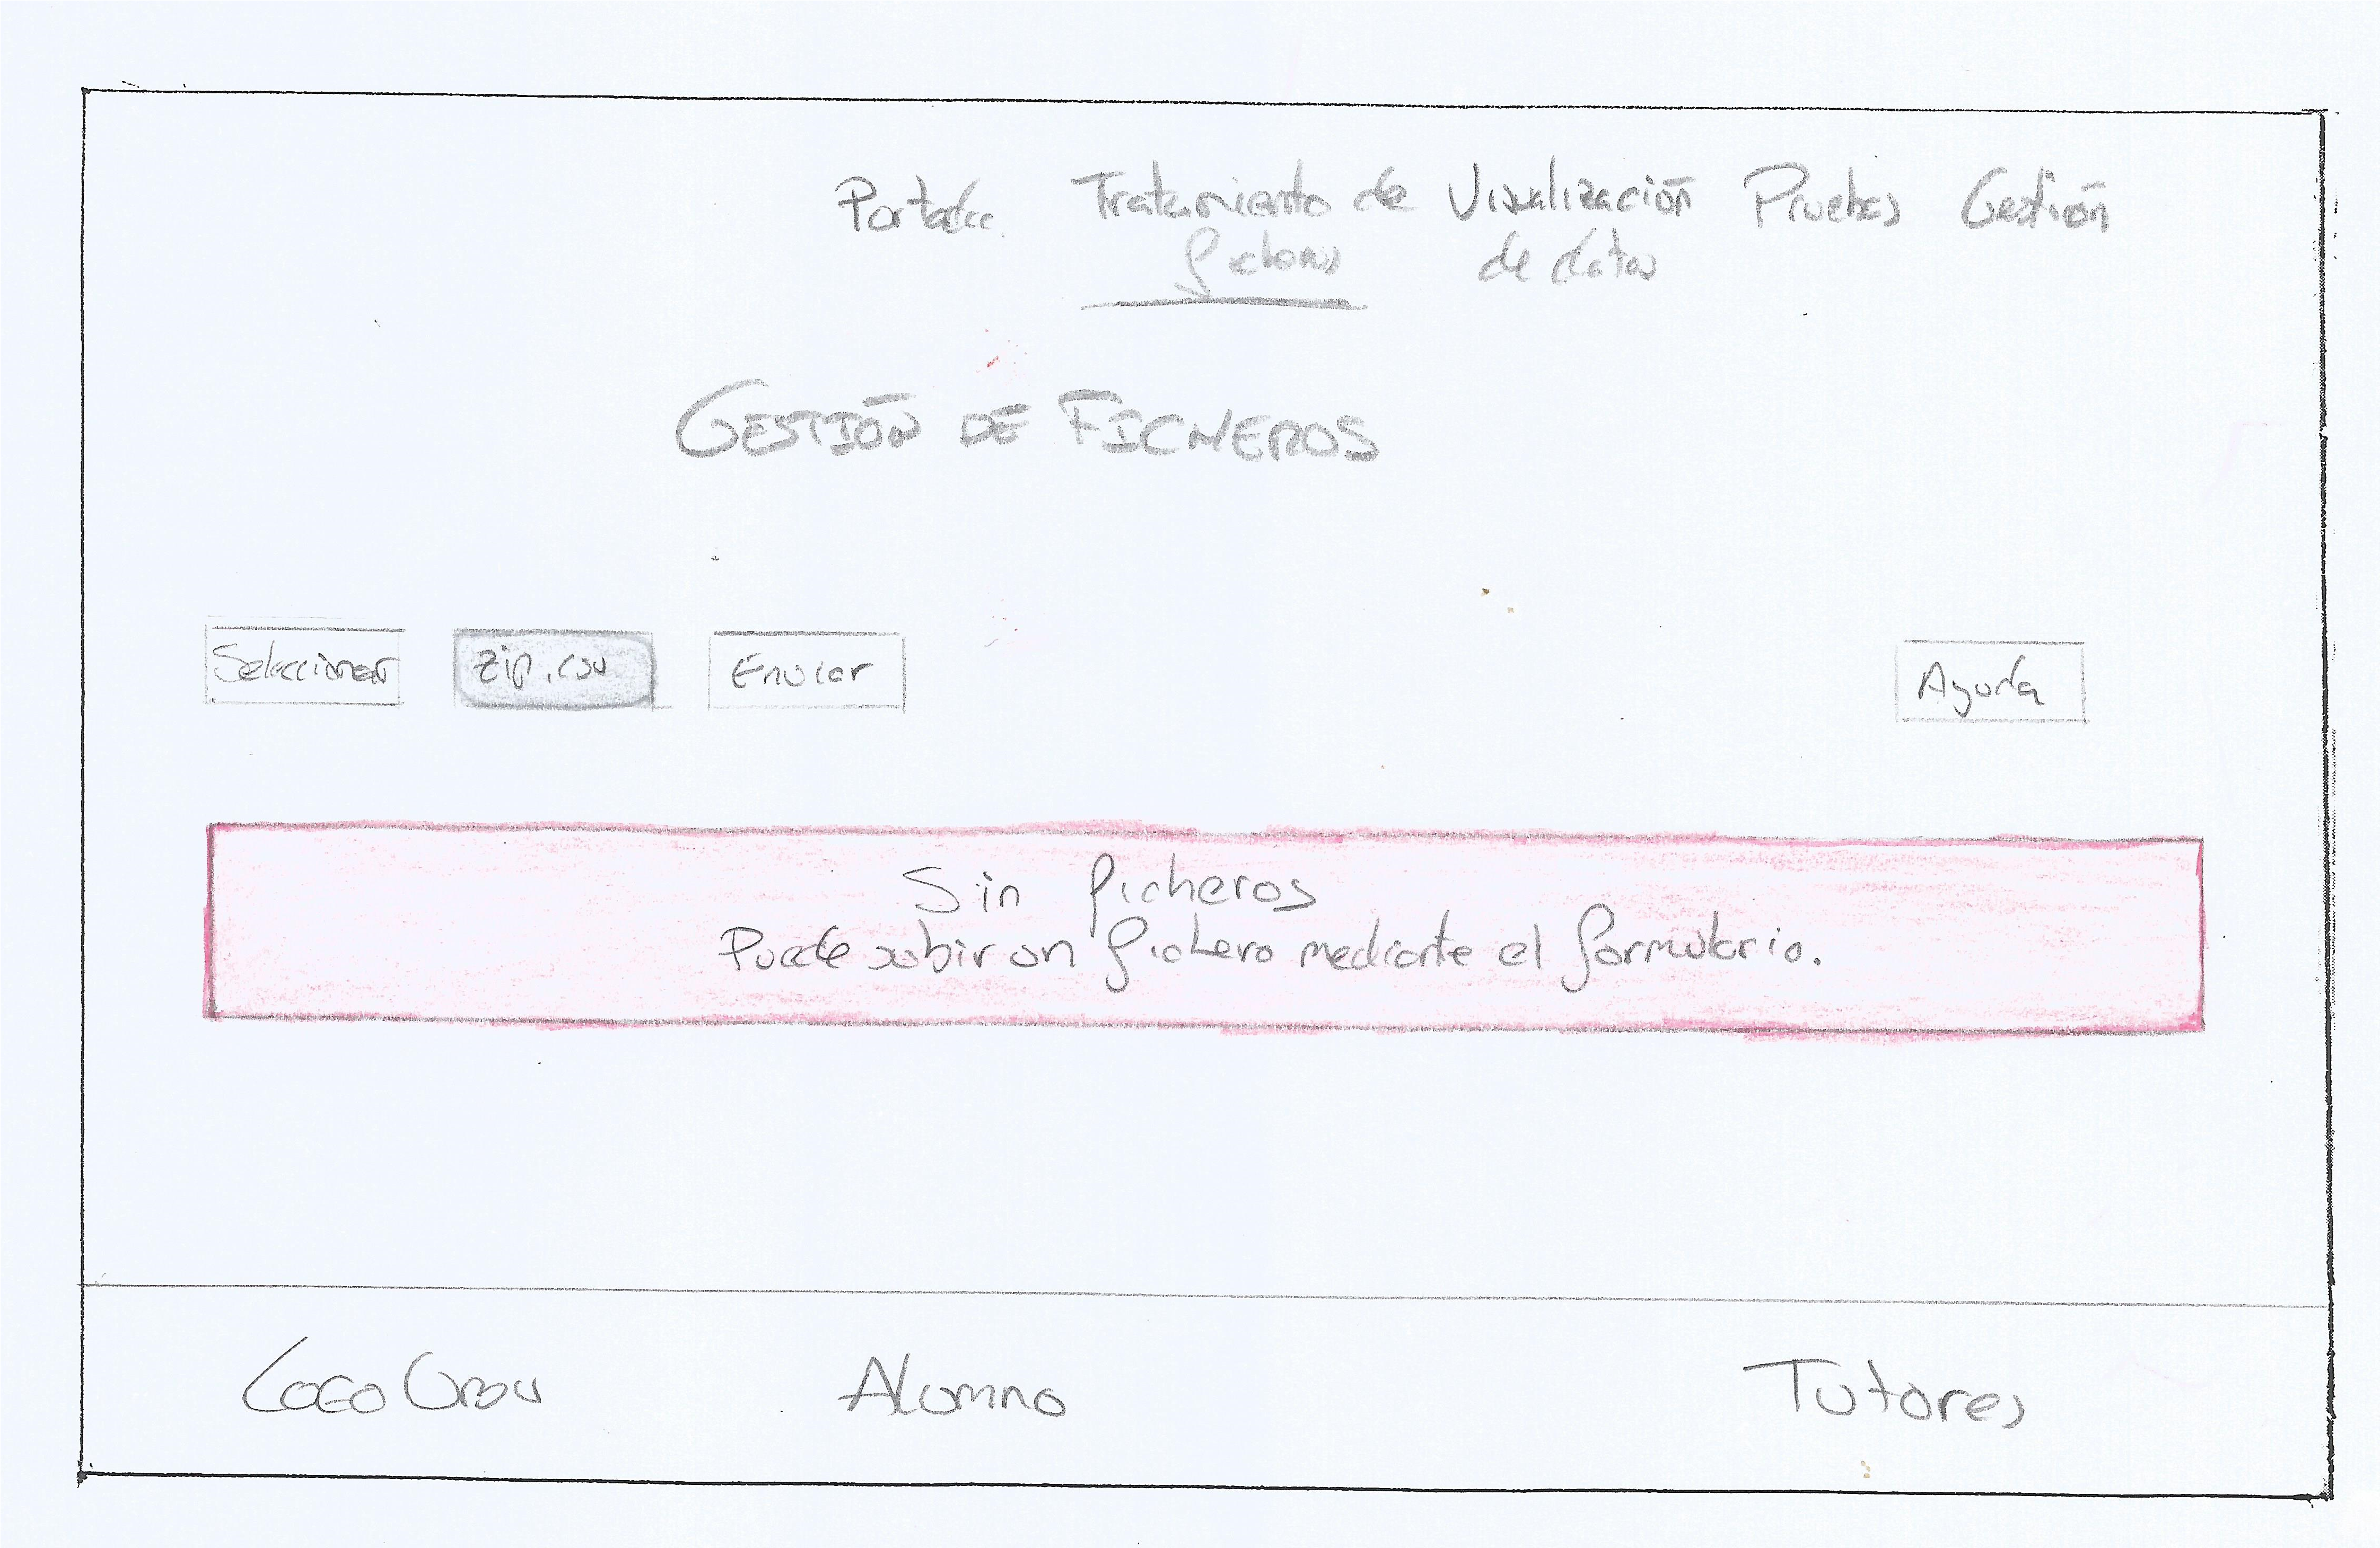
\includegraphics[width=0.8\textwidth]{../img/prototipado/alta/sinficheros.png}
  \caption{Aspecto de la página de ficheros, en esta caso, sin ficheros.}
  \label{sinficheros}
\end{figure}

\begin{figure}[!htbp]
  \centering
    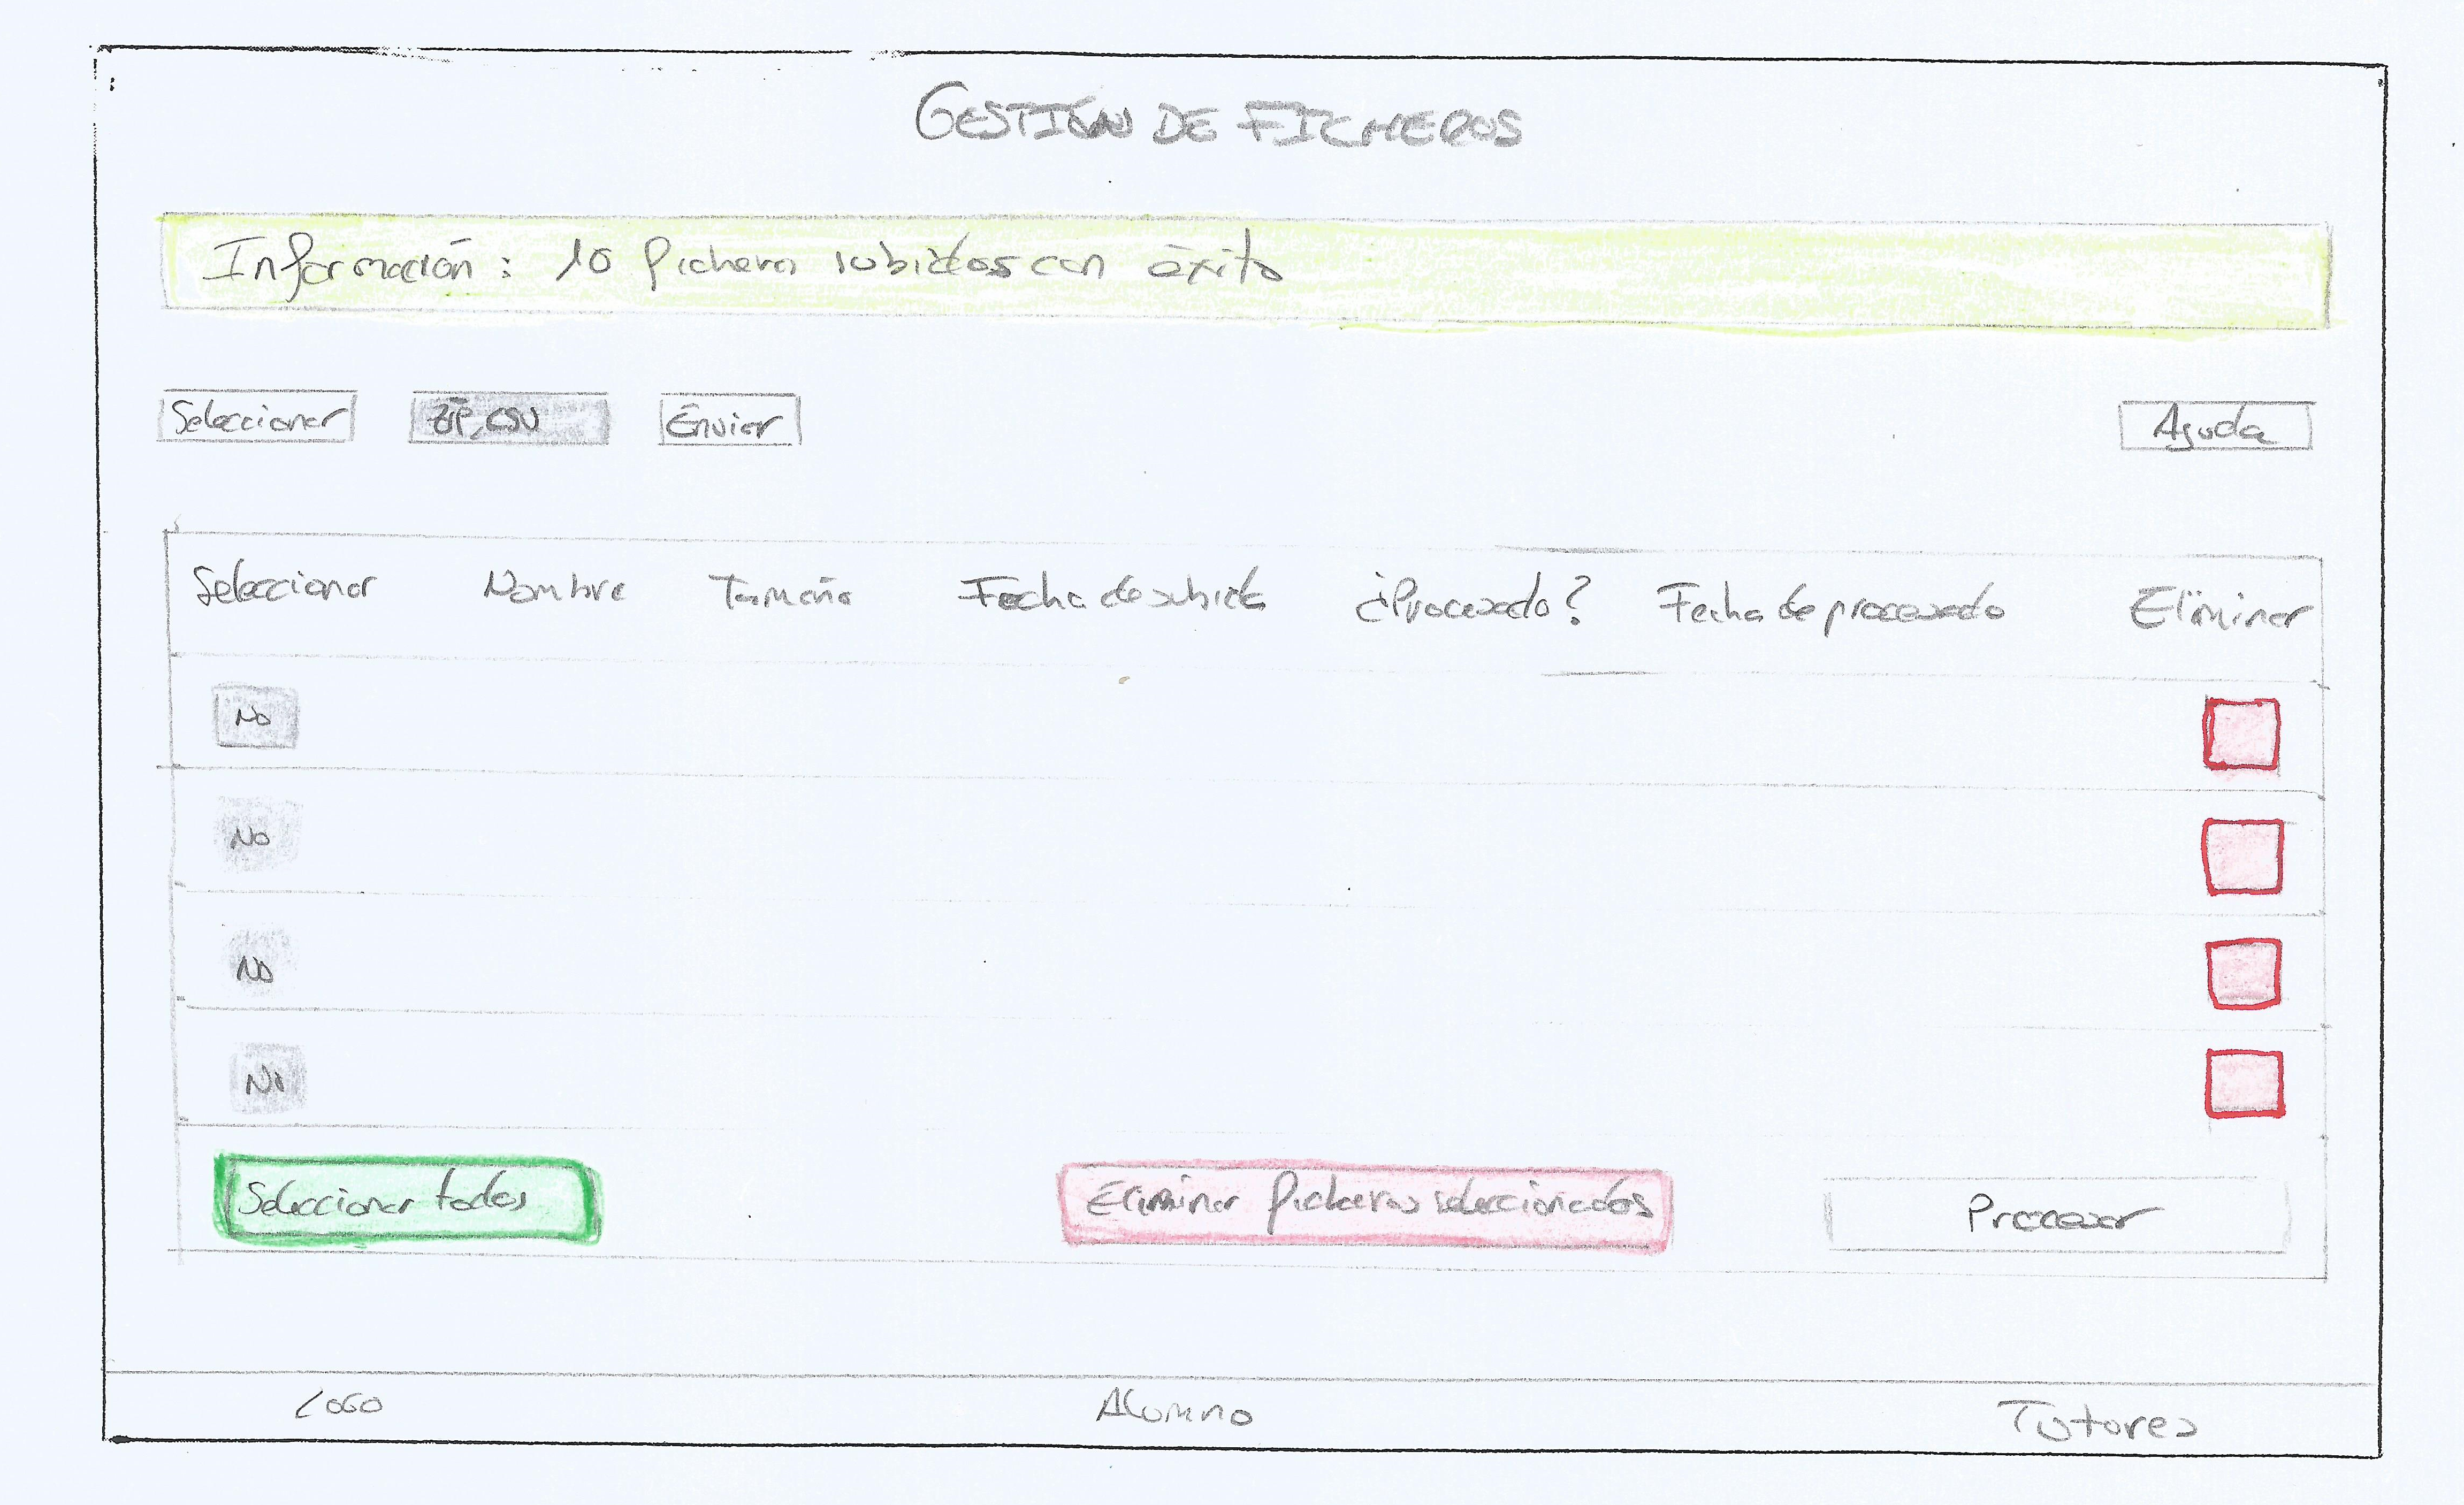
\includegraphics[width=0.8\textwidth]{../img/prototipado/alta/gestionficheros.png}
  \caption{Gestión de ficheros, algunos ficheros ya cargados.}
  \label{gestionficheros}
\end{figure}

\begin{figure}[!htbp]
  \centering
    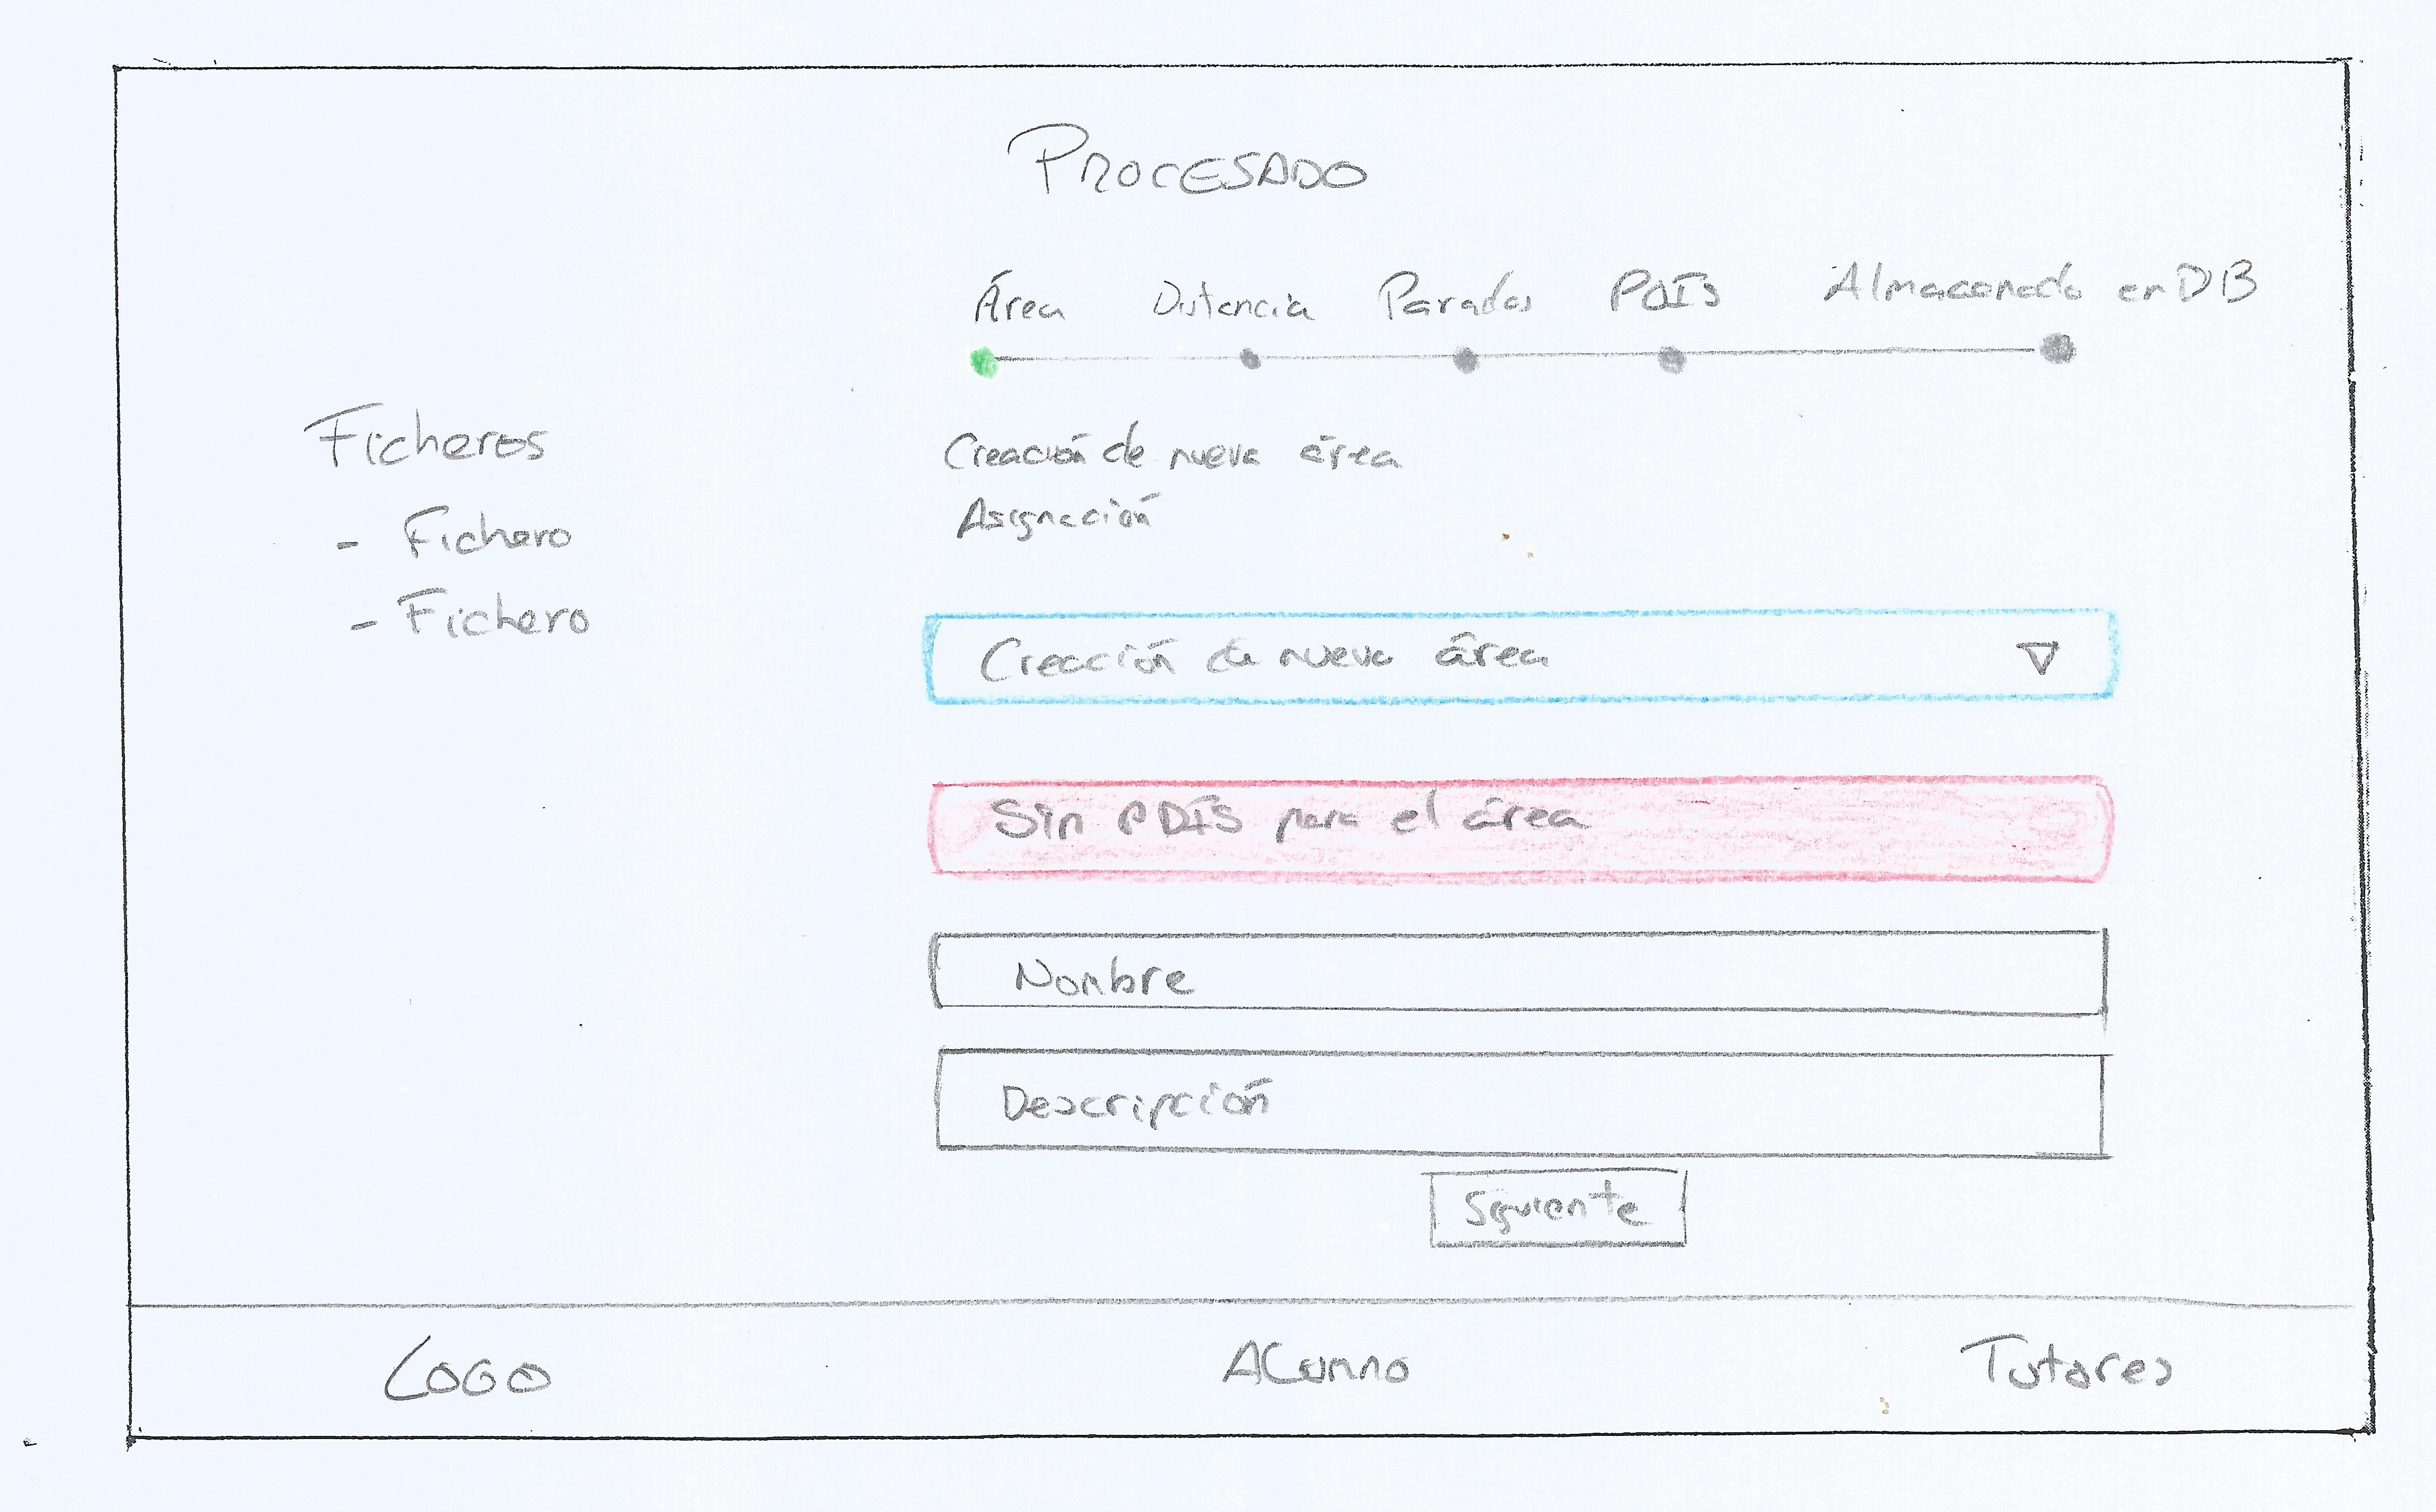
\includegraphics[width=0.8\textwidth]{../img/prototipado/alta/algoritmo.png}
  \caption{Opciones del algoritmo.}
  \label{algoritmo}
\end{figure}

\begin{figure}[!htbp]
  \centering
    \includegraphics[width=0.8\textwidth]{../img/prototipado/alta/encurso.png}
  \caption{Ejecución de una prueba en curso.}
  \label{encurso}
\end{figure}

\begin{figure}[!htbp]
  \centering
    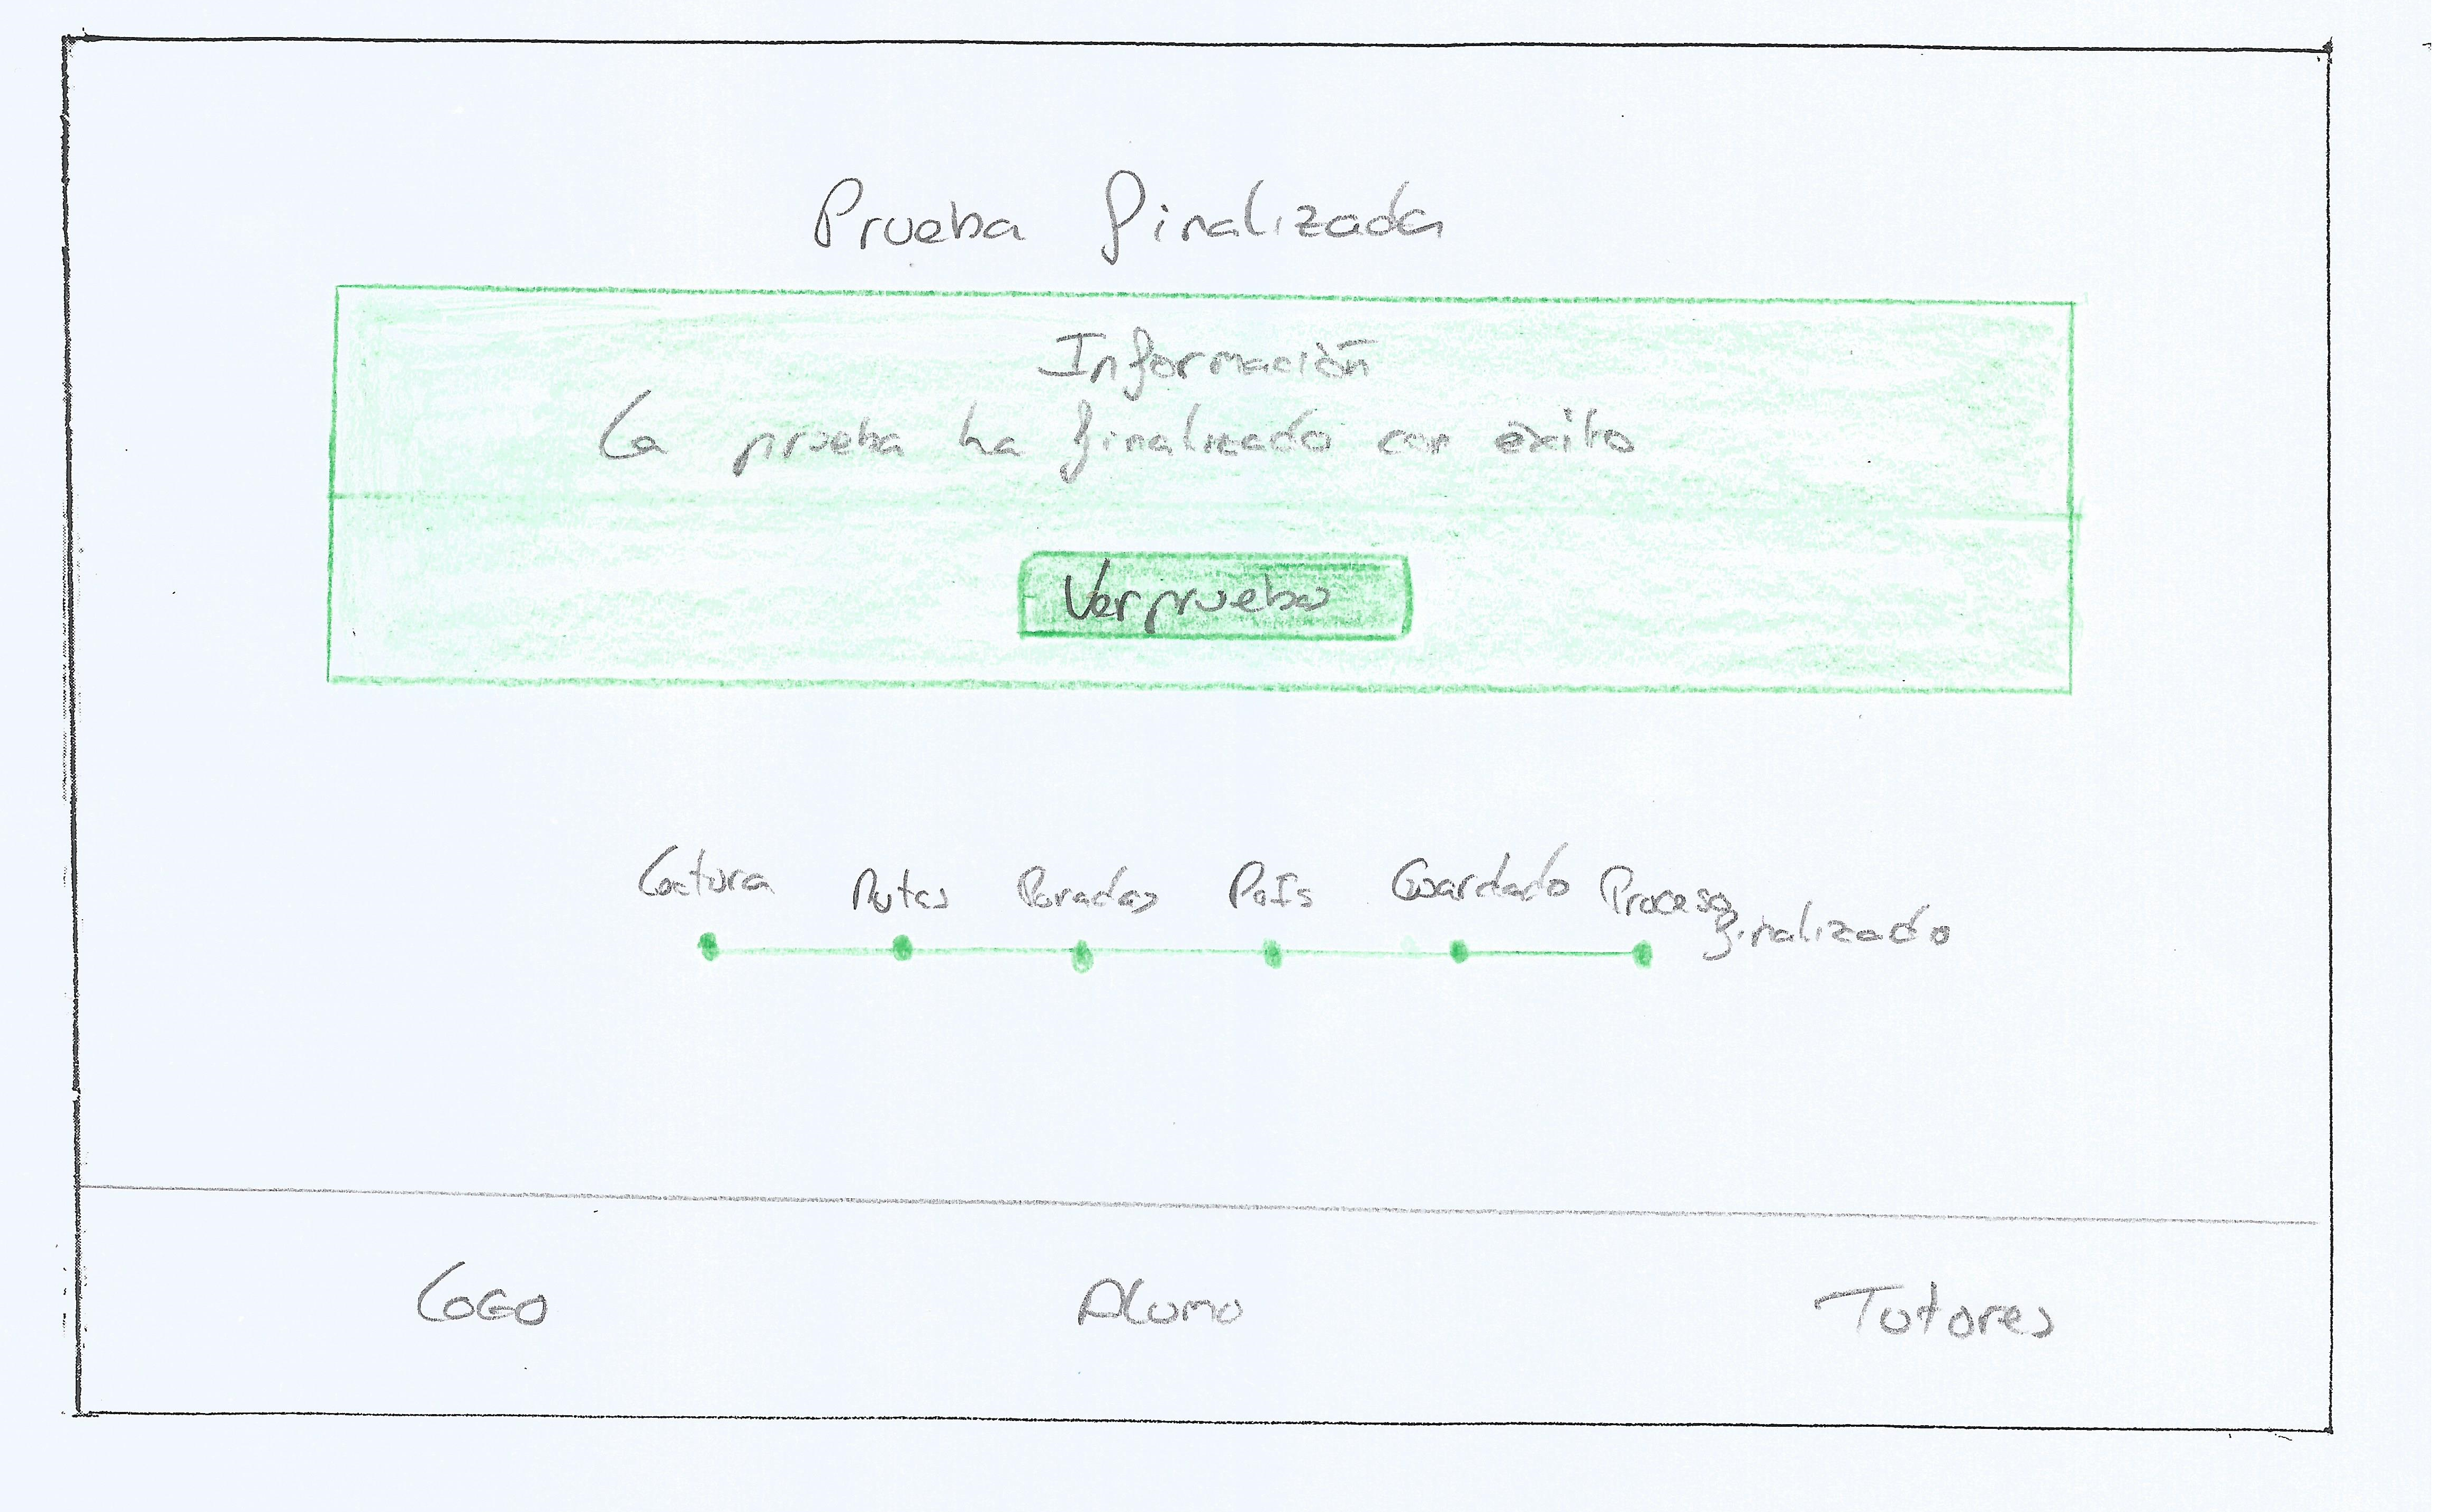
\includegraphics[width=0.8\textwidth]{../img/prototipado/alta/ejecucionfin.png}
  \caption{Ejecución finalizada.}
  \label{ejecucionfin}
\end{figure}

\begin{figure}[!htbp]
  \centering
    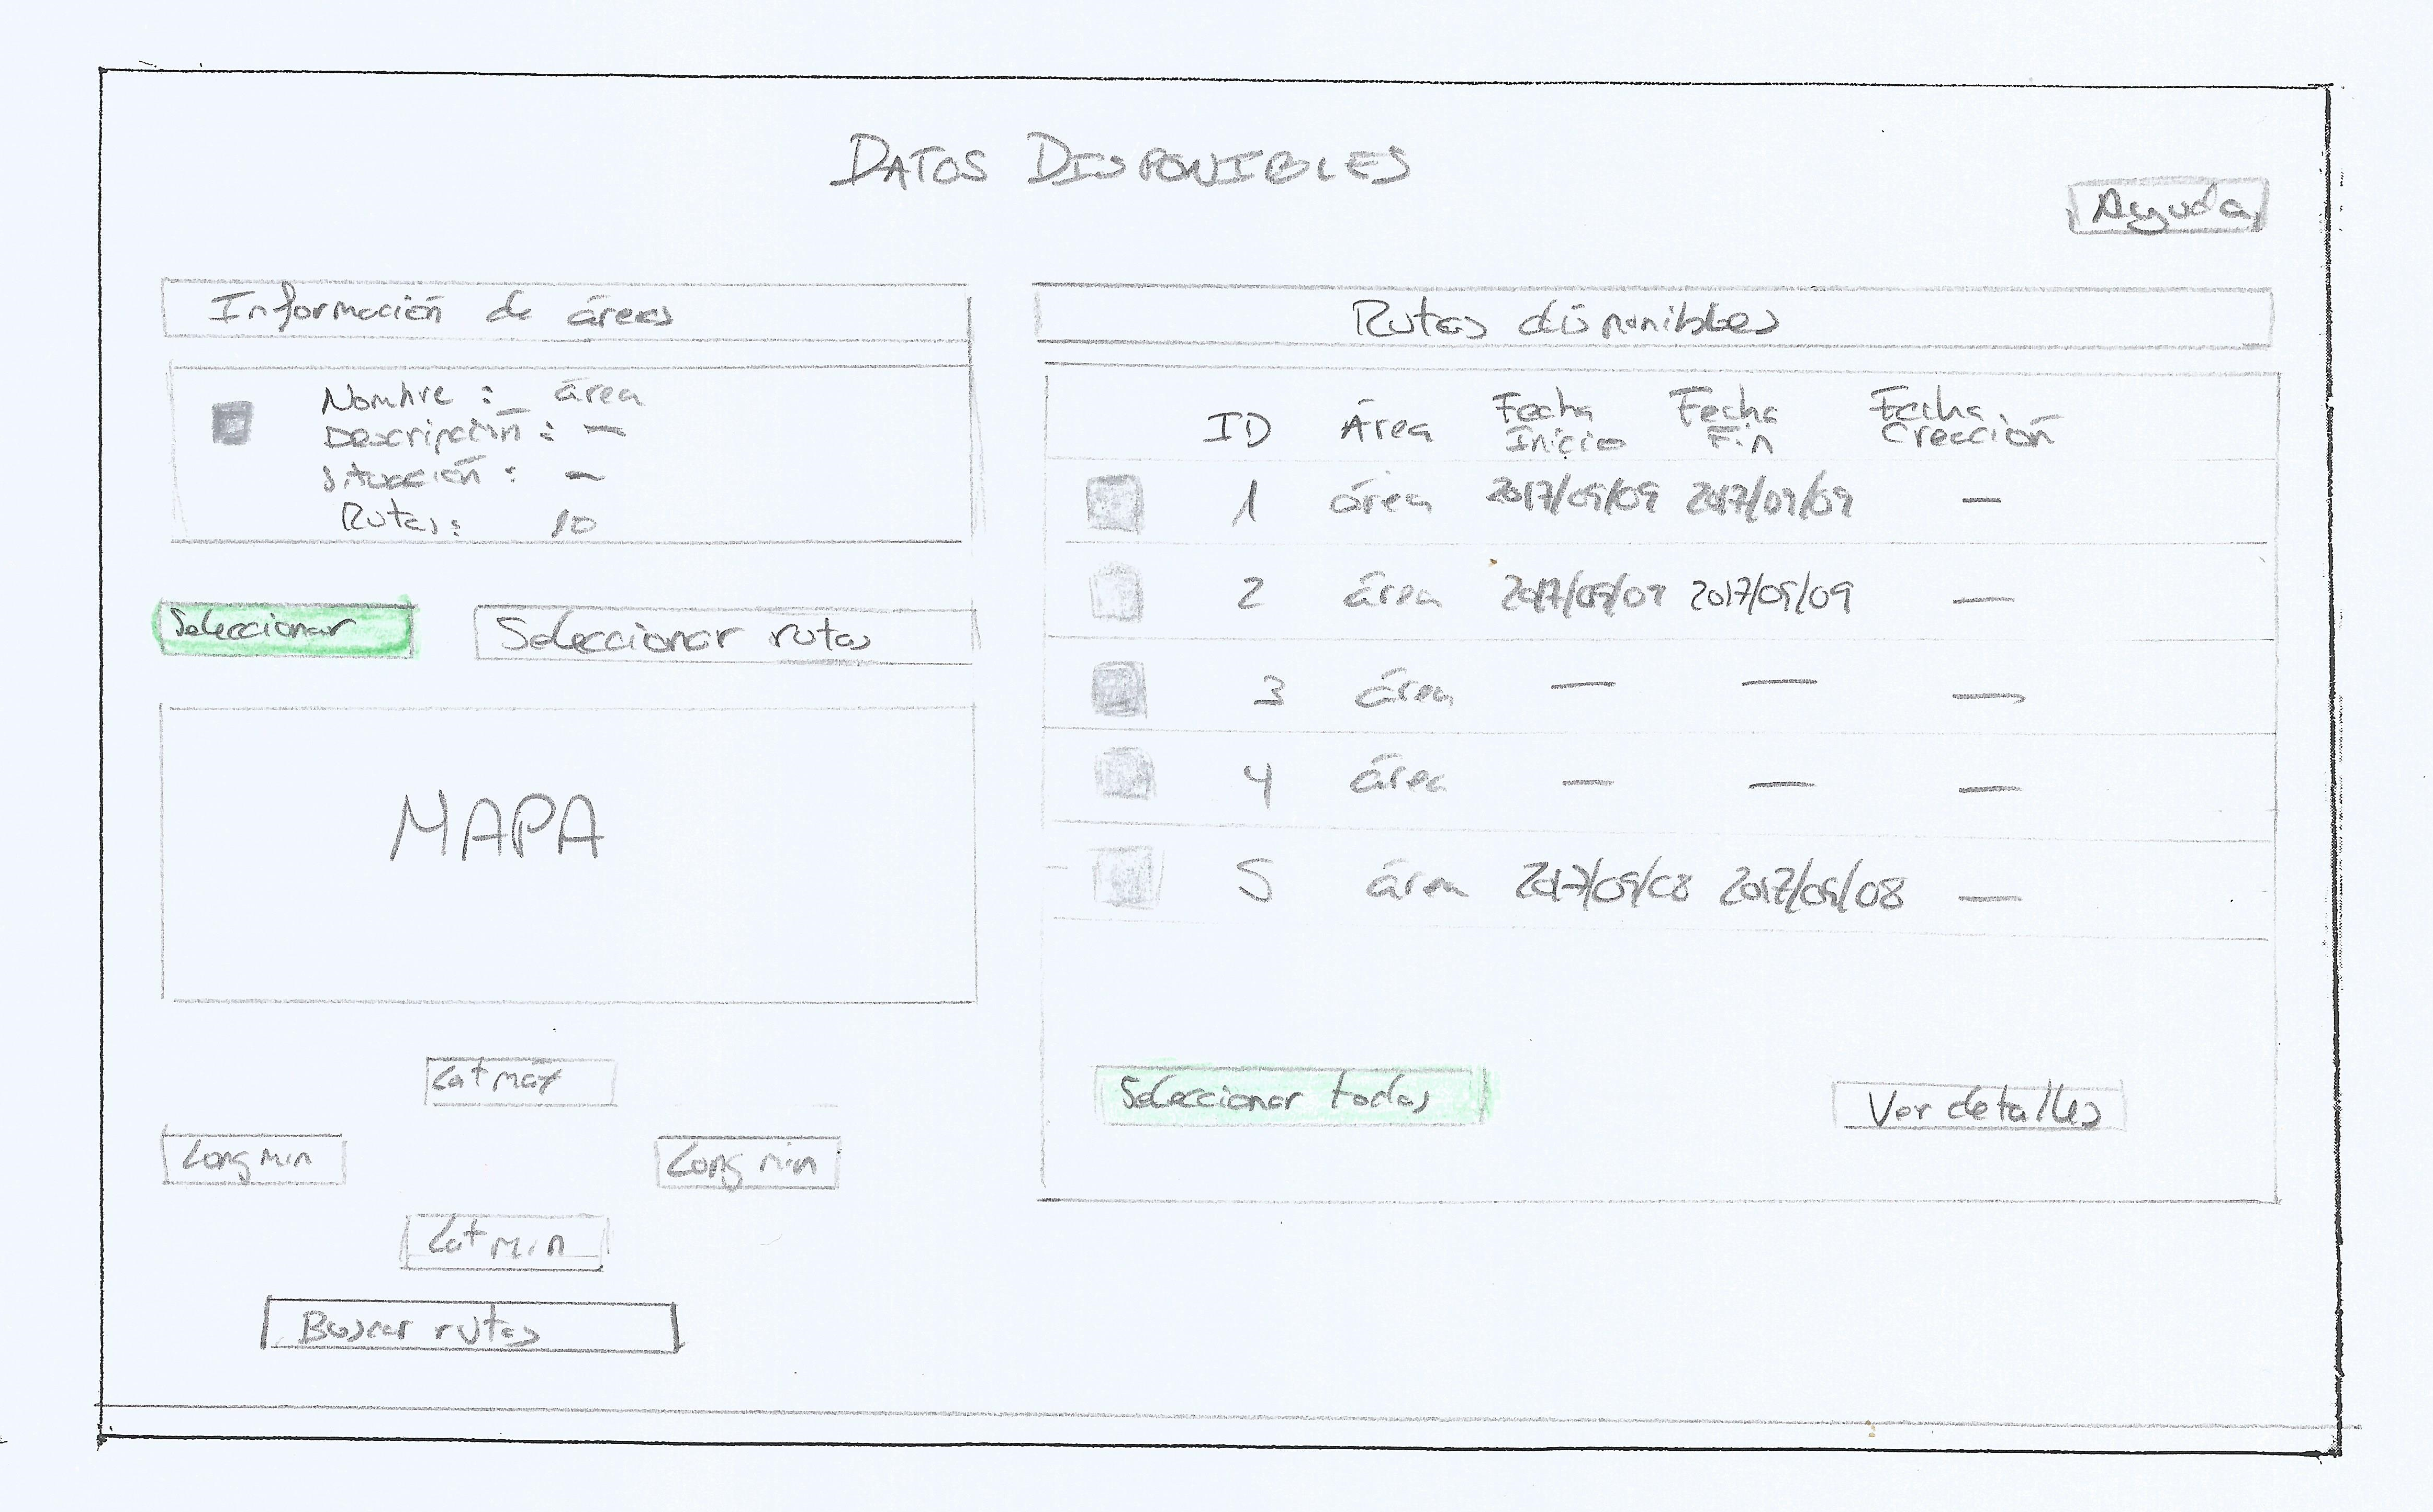
\includegraphics[width=0.8\textwidth]{../img/prototipado/alta/datosdisponibles.png}
  \caption{Áreas y rutas disponibles.}
  \label{datosdisponibles}
\end{figure}

\begin{figure}[!htbp]
  \centering
    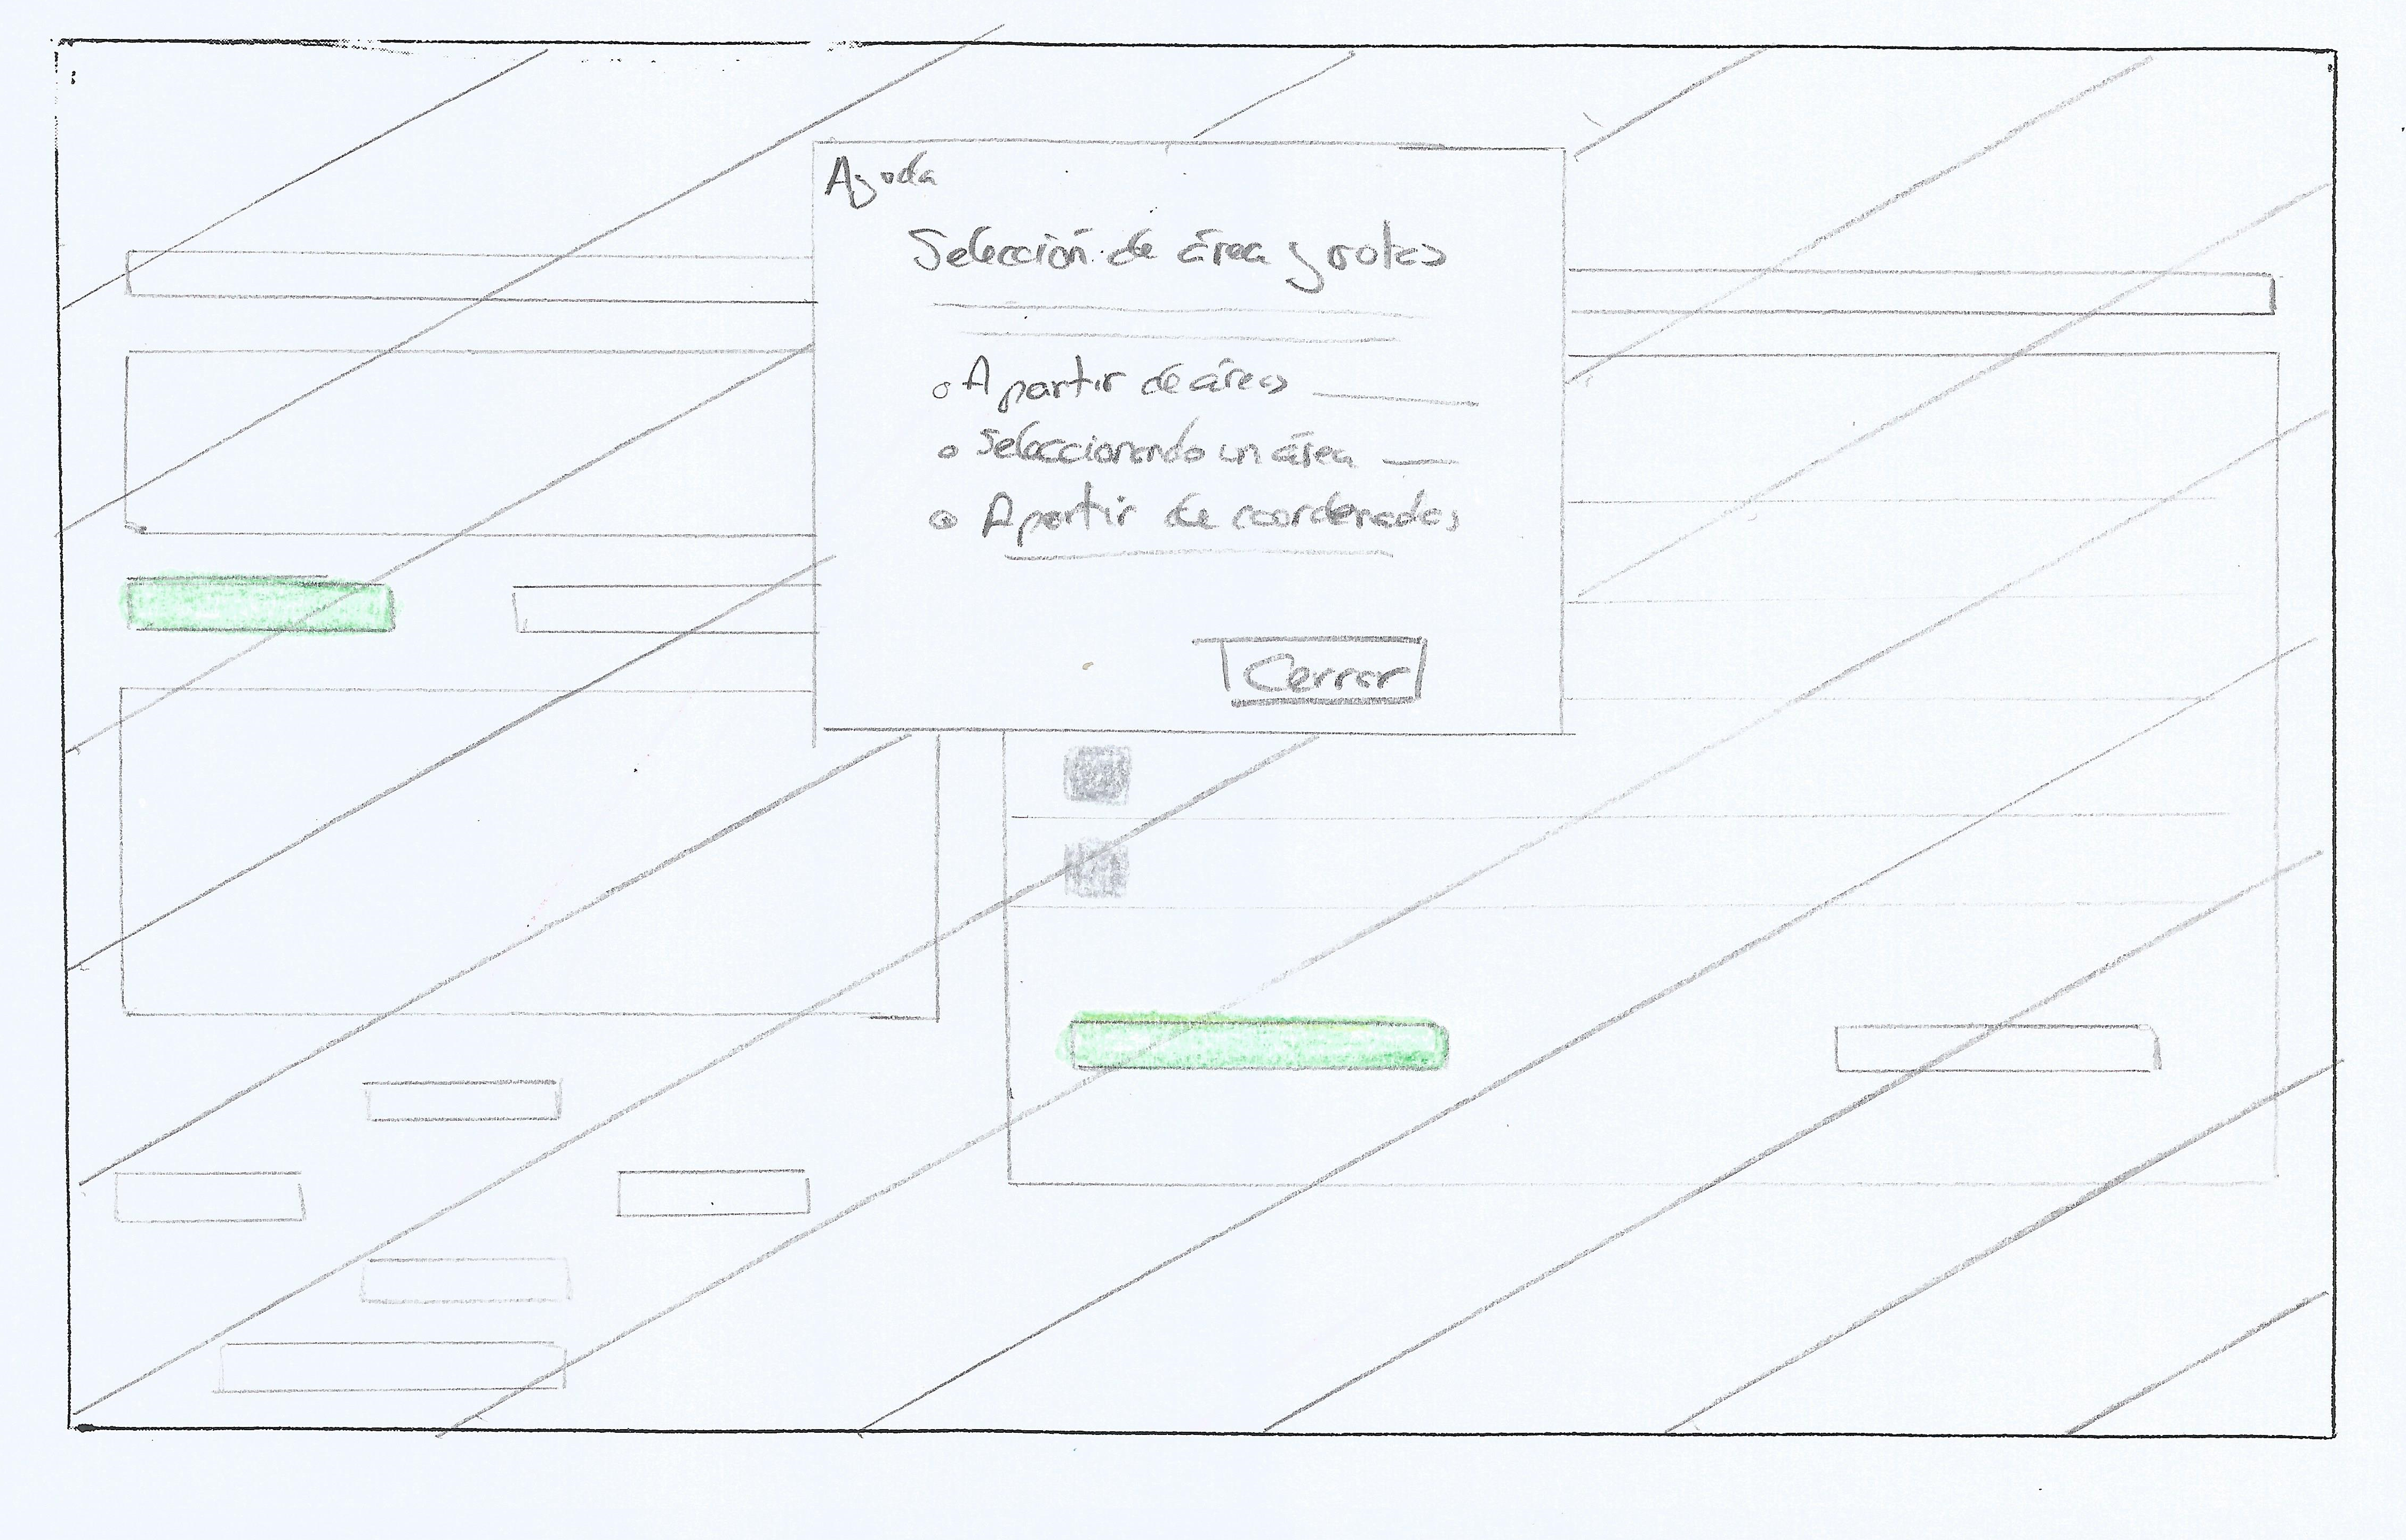
\includegraphics[width=0.8\textwidth]{../img/prototipado/alta/ayuda.png}
  \caption{Modales de ayuda, se puede encontrar ayuda en todas las páginas.}
  \label{ayuda}
\end{figure}

\begin{figure}[!htbp]
  \centering
    \includegraphics[width=0.8\textwidth]{../img/prototipado/alta/mapa.png}
  \caption{Las rutas podrán verse sobre un mapa.}
  \label{mapas}
\end{figure}

\begin{figure}[!htbp]
  \centering
    \includegraphics[width=0.8\textwidth]{../img/prototipado/alta/pruebas.png}
  \caption{Página de pruebas realizadas.}
  \label{pruebas}
\end{figure}

\begin{figure}[!htbp]
  \centering
    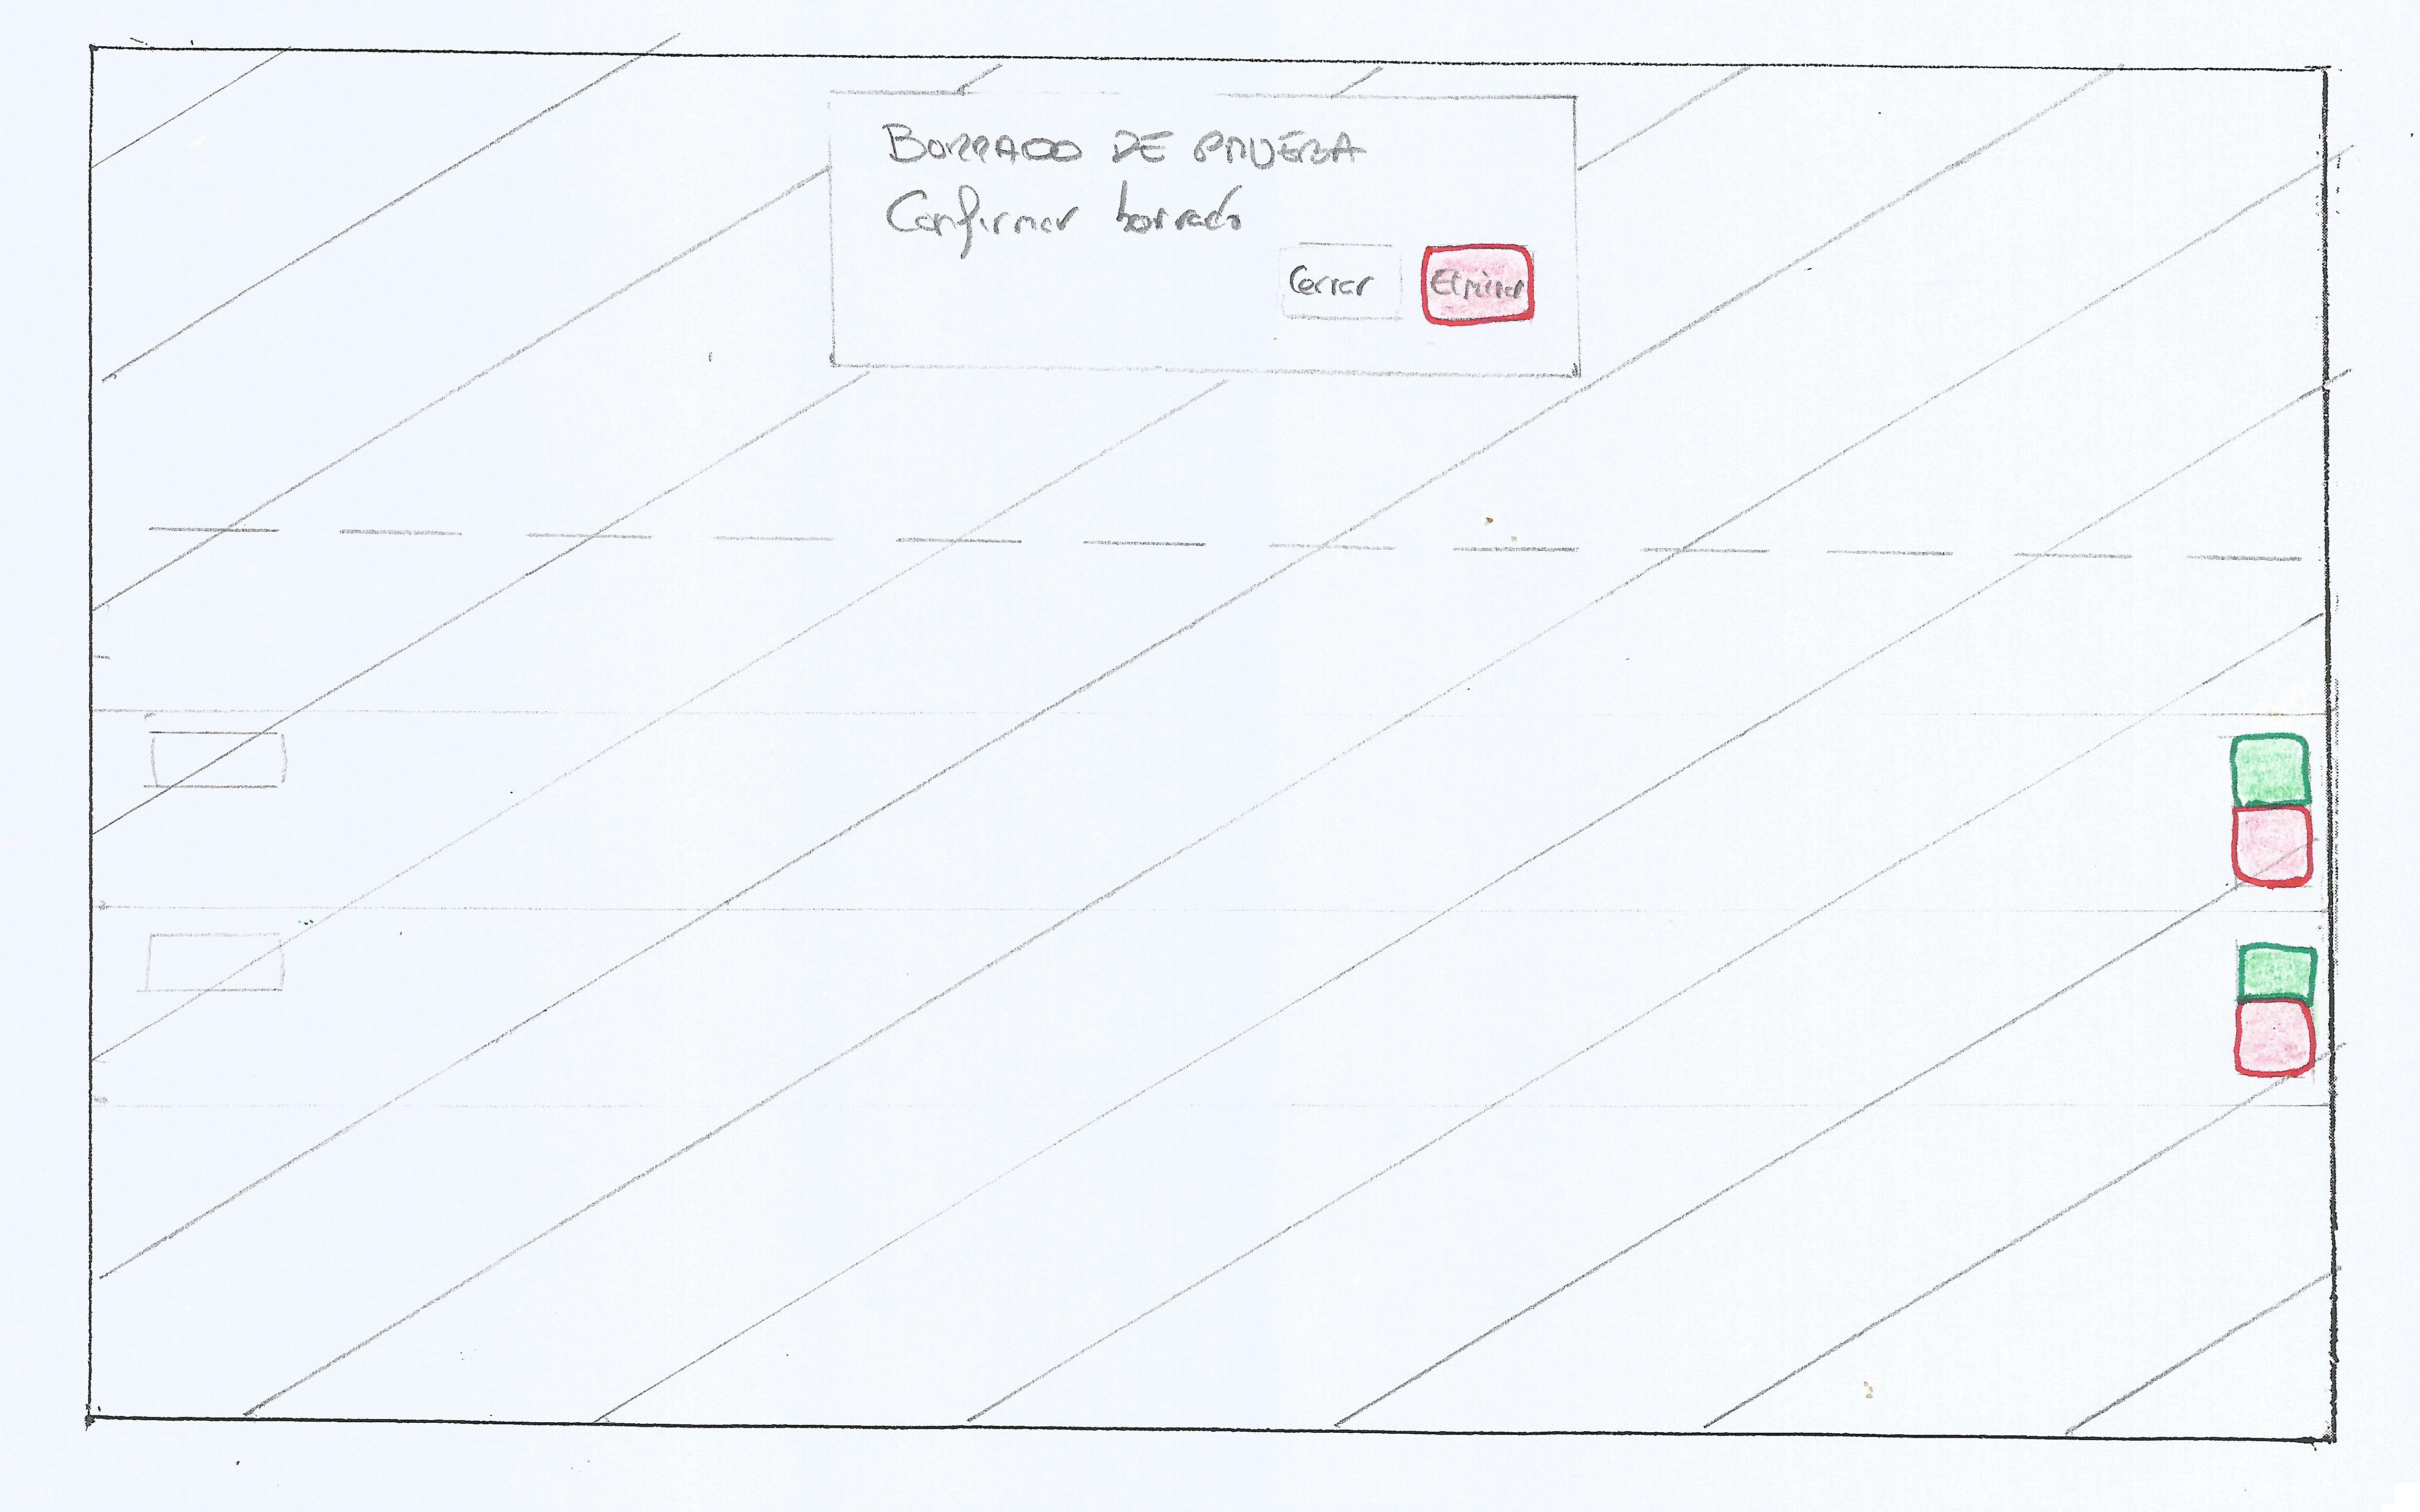
\includegraphics[width=0.8\textwidth]{../img/prototipado/alta/borradopruebas.png}
  \caption{Página de borrado de pruebas.}
  \label{borradopruebas}
\end{figure}

\begin{figure}[!htbp]
  \centering
    \includegraphics[width=0.8\textwidth]{../img/prototipado/alta/gestion.png}
  \caption{Página principal de gestión.}
  \label{gestion}
\end{figure}

\begin{figure}[!htbp]
  \centering
    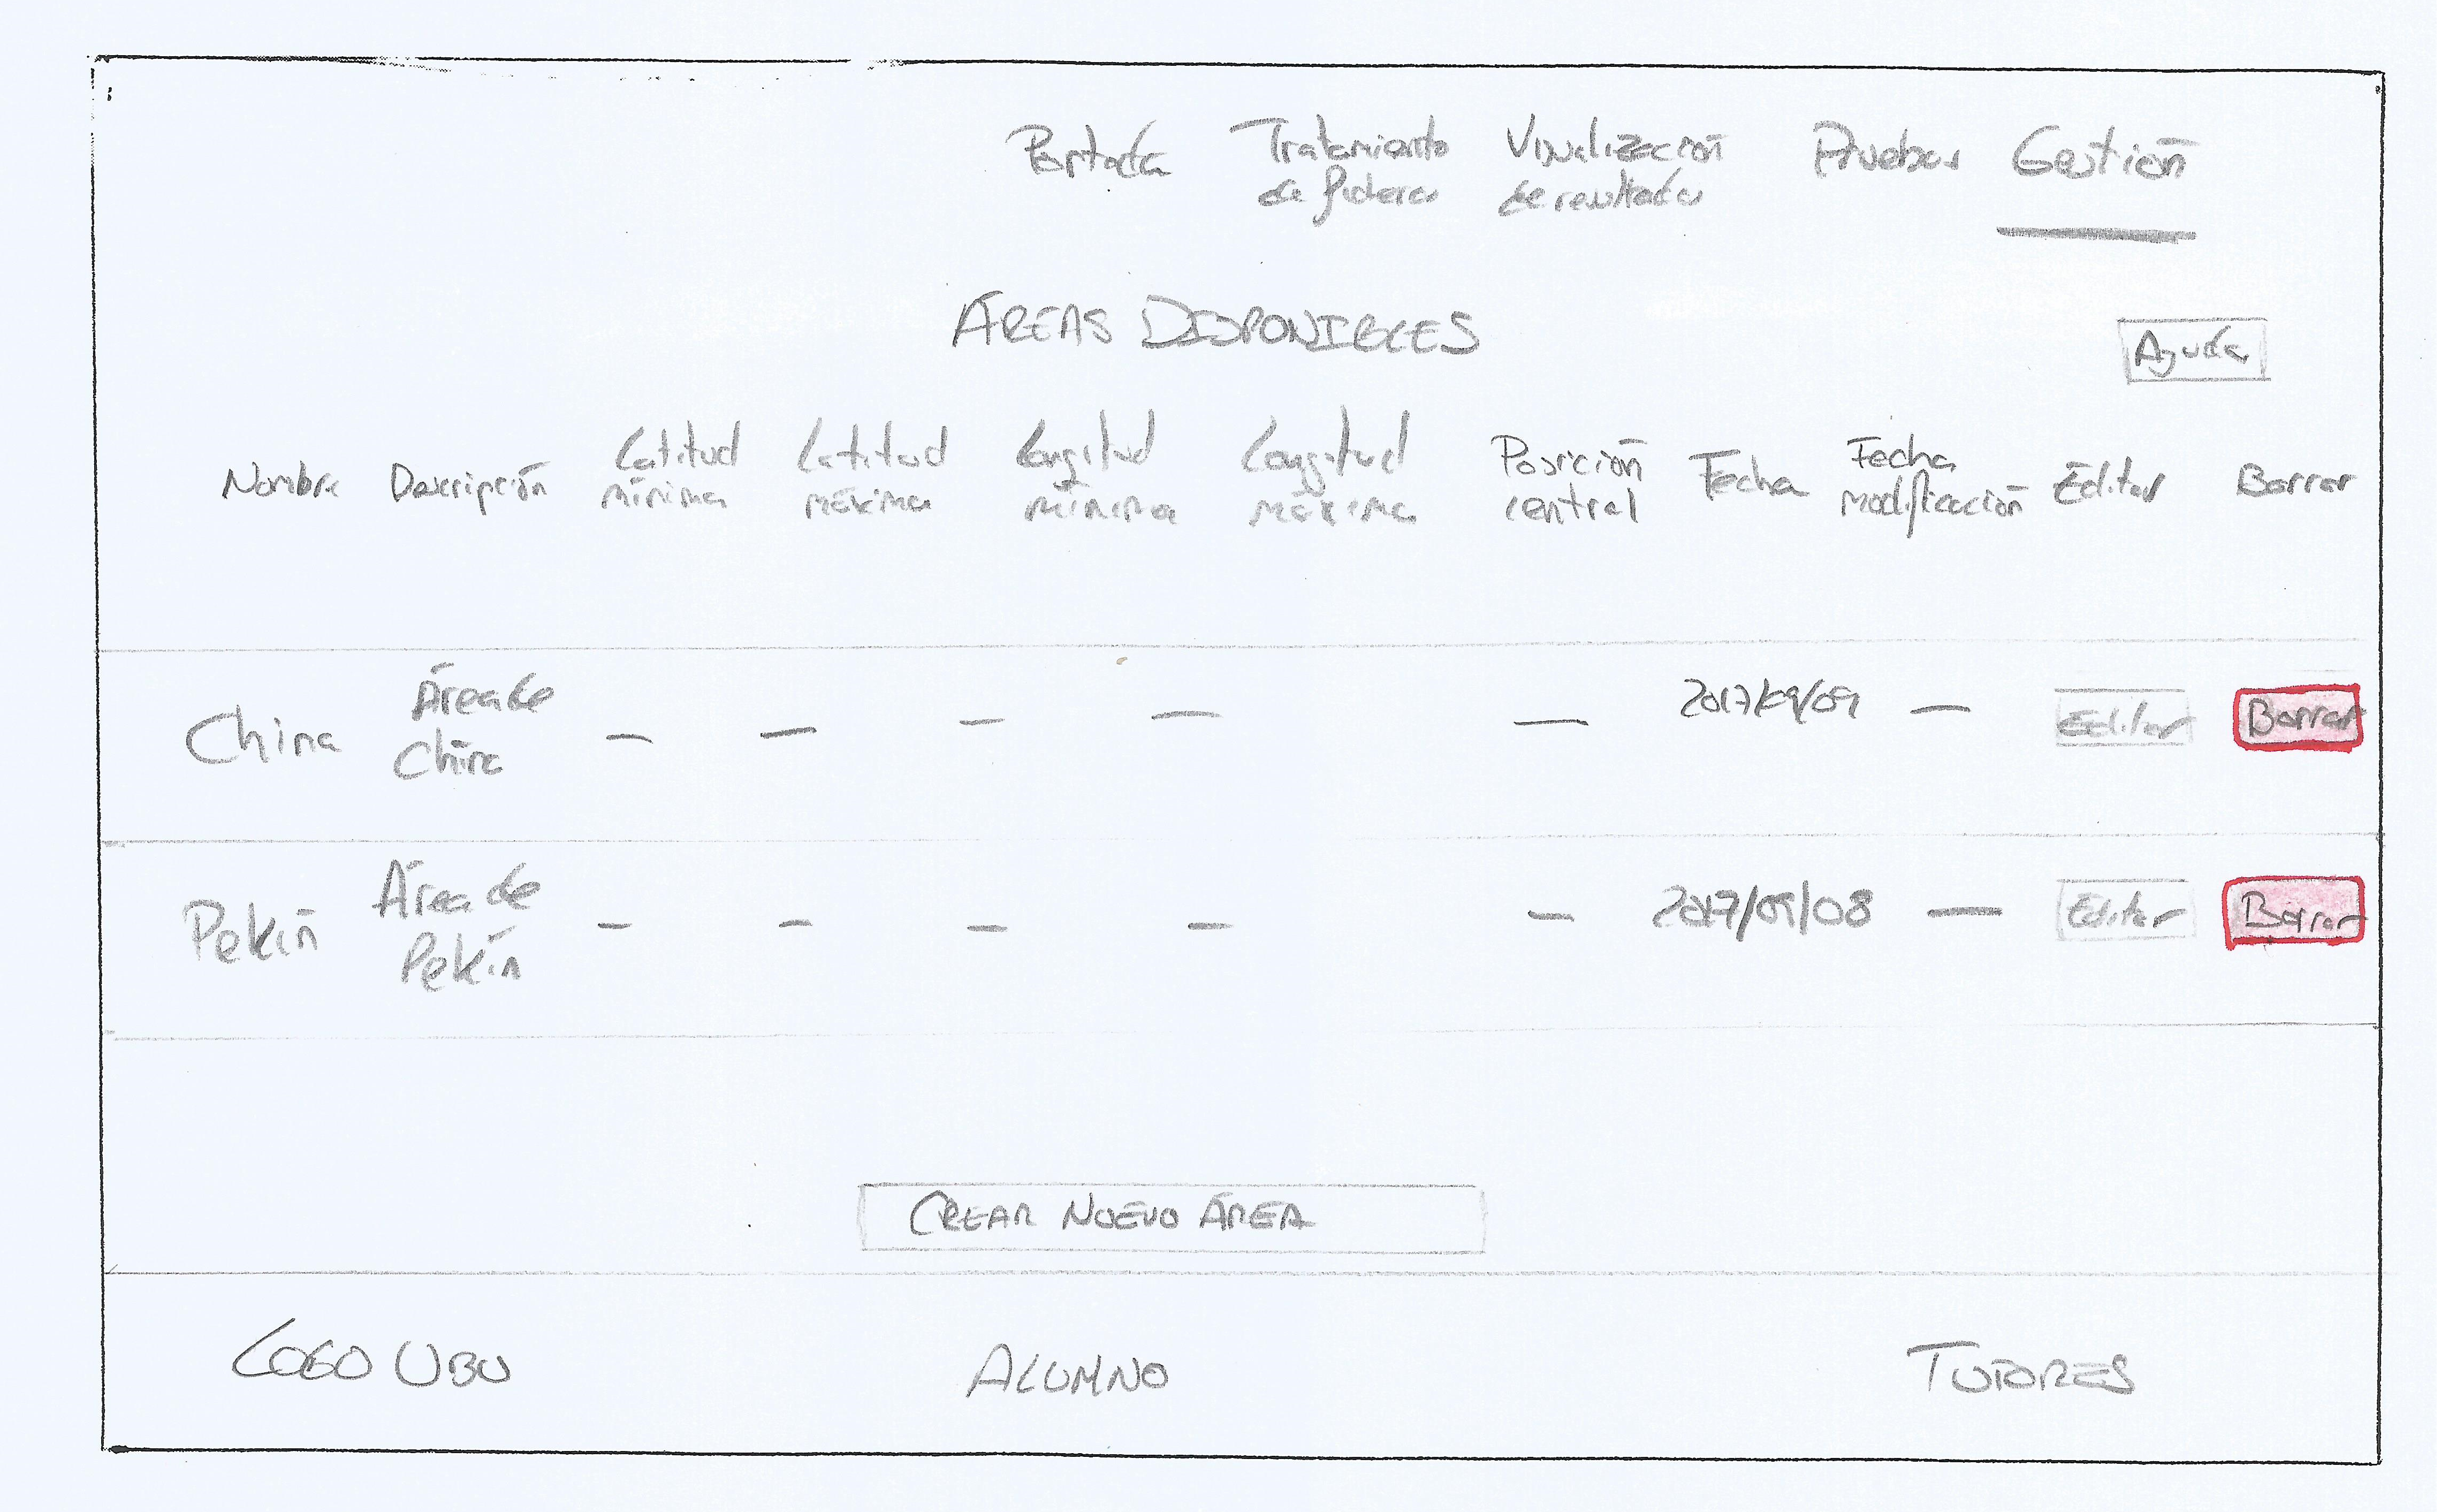
\includegraphics[width=0.8\textwidth]{../img/prototipado/alta/areasdispo.png}
  \caption{Página que muestra las areas disponibles en el sistema y que permite su mantenimiento.}
  \label{areasdispo}
\end{figure}

\begin{figure}[!htbp]
  \centering
    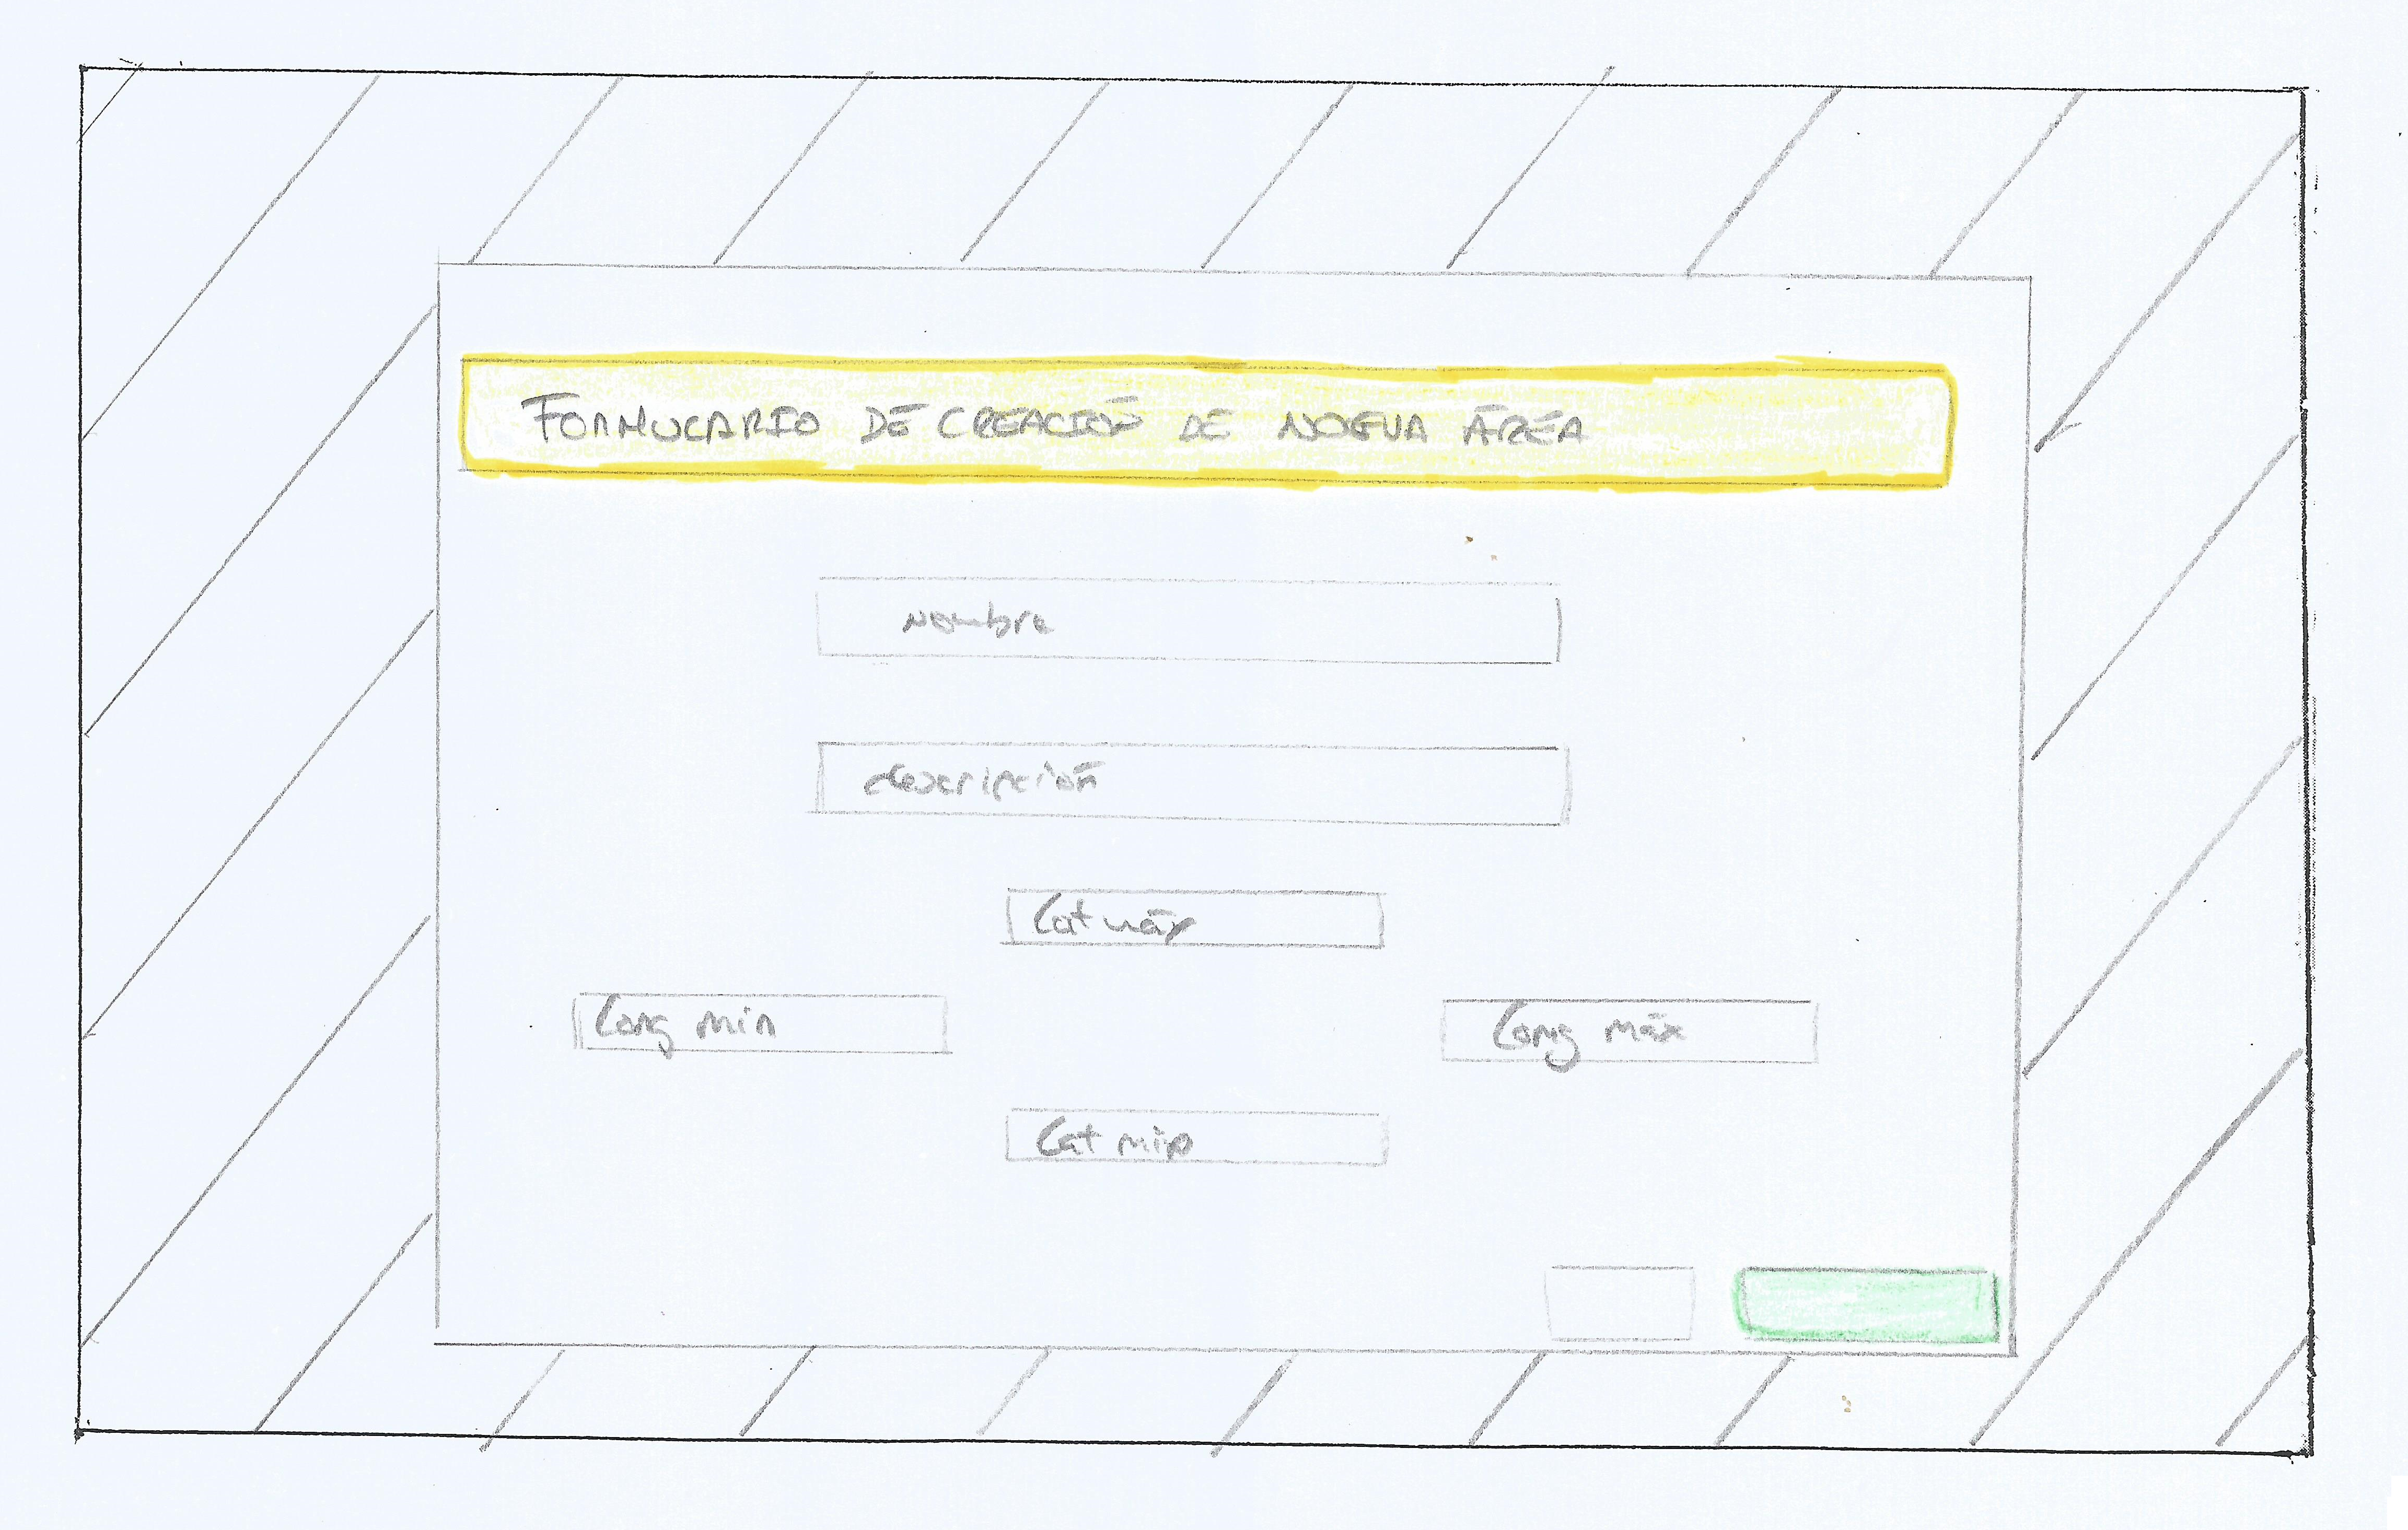
\includegraphics[width=0.8\textwidth]{../img/prototipado/alta/nuevaarea.png}
  \caption{Modal de creación de nueva área.}
  \label{nuevaarea}
\end{figure}

\begin{figure}[!htbp]
  \centering
    \includegraphics[width=0.8\textwidth]{../img/prototipado/alta/pdis.png}
  \caption{Gestión de PDIs.}
  \label{pdis}
\end{figure}

\begin{figure}[!htbp]
  \centering
    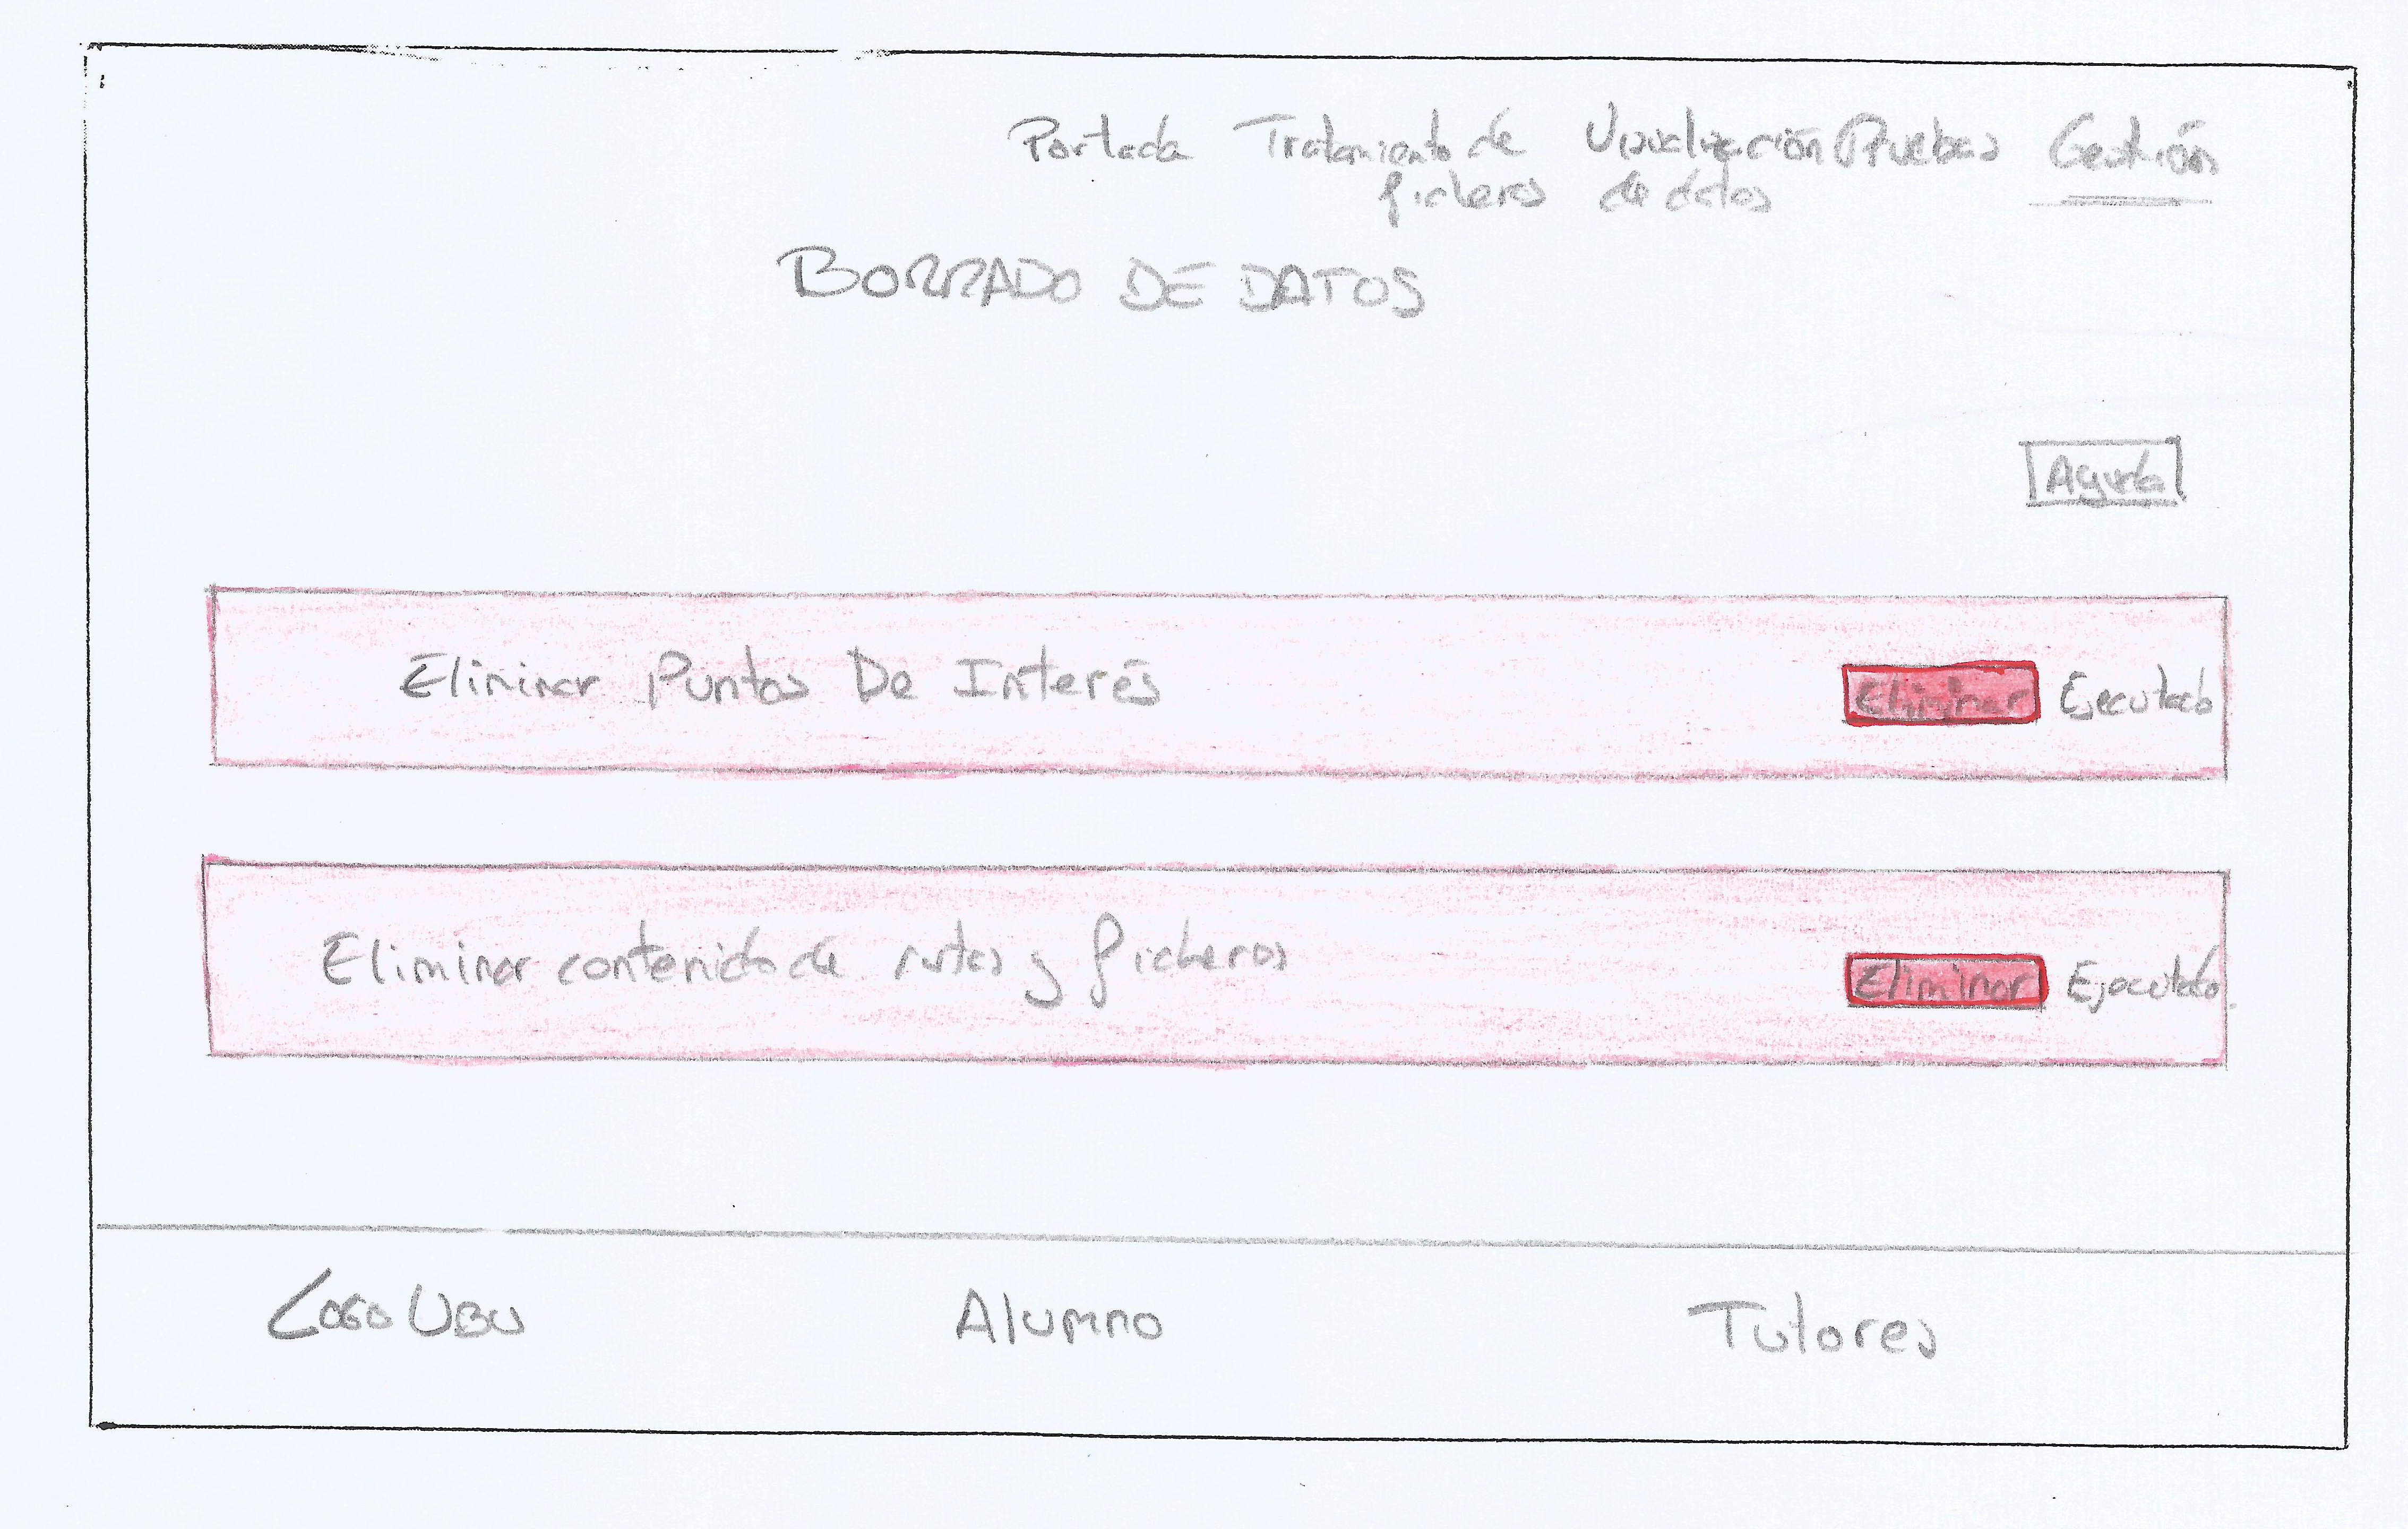
\includegraphics[width=0.8\textwidth]{../img/prototipado/alta/borrado.png}
  \caption{Página de borrado de datos.}
  \label{borrado}
\end{figure}
